\documentclass[10pt]{article}
\usepackage[margin=0.75in]{geometry}
\usepackage{graphicx,booktabs,amsmath,float}
\usepackage[font=small]{caption}
\begin{document}
\begin{center}{\Large\bf Feature importance of the 15:30 forecast (16:00 bar)\\ re-run on the de-duplicated per-bar design}\\[3pt]
{\small MDI, split count, permutation importance on the causal held-out tail, SHAP --- trees and the per-bar linear models; 1,469 forecasts 2018-06-25 .. 2024-04-30, 147 refits}\end{center}

\textbf{What changed from the first pass.} (i) The design: the per-bar design no longer carries the twelve HAR$\times$open/close session-edge interactions (at 16:00 the six \texttt{har\_ma\_k\_x\_open} columns were all zero and the six \texttt{har\_ma\_k\_x\_close} columns exact copies of \texttt{har\_ma\_1 .. har\_ma\_3125}); columns HAR + calendar 34$\to$22, live-feasible 244$\to$232, all features 640$\to$628. (ii) The trees: every tree fit uses only the columns kept by the per-window mask of its own 2000-session training window (constant columns and exact copies removed; the linear arms' identifiability mask applied to the trees); MDI, split count and TreeSHAP are mapped back to all columns with 0 for a dropped column, and permuting a dropped column changes nothing. Kept columns per refit (min / median / max): HAR + calendar 17 / 17 / 17 of 22; live-feasible 136 / 138 / 145 of 232; all features 360 / 369 / 378 of 628. The linear models are unchanged by the mask (theirs already removed these columns at every tune). Everything else is the first pass's (147 refits, the same held-out tails, permutation generator and seeds, models and parameters), so before/after differs only by the design and the mask --- and by the permutation draws of most units (the stream is laid out unit by unit and the unit count changed: a column's P1 draws are identical in both runs, the P2 draws and the group units' draws are fresh; the ridge fits are the same problem in both runs, so the ridge rows measure that Monte Carlo noise). (iii) Cadence: the campaign's trees now refit every session; at an importance refit the model is identical under either cadence (same window, same configuration), so the importance at every 10th refit is the daily-refit model's importance on those days (Section 8). Before/after rankings: Section 9.

\textbf{Setup.} Models: per-bar ridge and lasso (coefficients re-solved every session, penalty re-chosen causally every 250 sessions) and the untuned per-bar LightGBM, XGBoost and random forest (refit every 10 sessions) --- the shipped configurations. Every fit uses the 2000 sessions before it. A refit's \emph{held-out tail} is the $\le 10$ sessions its model forecasts, up to the next refit: never in its fit, so a loss change measured there is out of sample and causal. Buckets: live-feasible (the deck's), all features, and HAR + calendar. Library: scikit-learn 1.9.0 (random forest), LightGBM 4.6.0, XGBoost 3.2.0, shap 0.51.0; the permutation and drop-column loops are written out, because a library permutation routine scores one fitted model on one test set, not 147 walk-forward models on their own tails.

\textbf{Measures.} (1) \emph{MDI / gain}: LightGBM gain, XGBoost total gain, random-forest impurity decrease; share per refit, averaged. (2) \emph{Split count}. (3) \emph{Permutation importance} on the tail, loss = QLIKE of the plain back-transform $\hat y^2\times$ diurnal baseline against the bar's realized variance (no recalibration), and squared error in the fit space; 10 draws per unit and refit, the same draws for all five models. P1 shuffles the unit's values among the tail's rows (the literal permutation; blind to slow inputs, which barely move in 10 sessions); P2 replaces them with rows drawn from the refit's own training window (past data only). A unit is a column, a \emph{series} (all columns of one input: lags, flags, gates) or a \emph{cluster} (columns every pair of which has $|$corr$|\ge 0.8$, complete linkage); a group's columns move together. Intervals: 95\% circular-block bootstrap over refits (block 6). (4) \emph{SHAP}: TreeSHAP (path-dependent) on the same tail rows; for the linear models $\beta_j(x_j-\bar x_j)$ with the window mean as background. Linear extras: $|\beta\cdot sd|$ and drop-column importance (re-solve without the unit, penalty held).

\textbf{Key.} \texttt{har\_ma\_*} realized variance of the bar (the target's own HAR ladder, means over the last 1, 5, 25, 125, 625, 3125 bars; the per-bar design no longer carries the session-edge interactions \texttt{har\_ma\_*\_x\_open/close}); \texttt{adj\_sumabsret\_ma\_*} absolute return; \texttt{adj\_sumret\_ma\_*} signed return; \texttt{adj\_sumret3/4\_ma\_*} 3rd/4th-power returns; \texttt{adj\_sumpret2\_ma\_*} upside squared returns; \texttt{adj\_sumbipow\_ma\_*} bipower variation; \texttt{adj\_sumautocov\_ma\_*} return autocovariance; \texttt{adj\_sumvolume\_ma\_*} ES volume; \texttt{adj\_numobs\_ma\_*} ES prints per bar; \texttt{adj\_vix/vvix/vix3m\_ma\_*} the Cboe indices; \texttt{adj\_fomc\_*} FOMC flags and distances; \texttt{*\_avail/active\_ma\_*} is-present / is-nonzero flags; calendar = \texttt{DOW\_*}, \texttt{is\_*}, \texttt{hour}, \texttt{days\_to\_opex}. all features adds the constituent cross-section (\texttt{*\_ewstock}, \texttt{*\_vwstock}), Cboe volume (\texttt{adj\_voldemand\_*}) and StockTwits (\texttt{adj\_stocktwits\_*}).

\begin{table}[H]\centering\footnotesize
\caption{The design is float throughout, but not all continuous: distinct values per column in each 2000-session window (median over the 147 windows) --- what MDI's cardinality bias keys on.}
\begin{tabular}{lrrrrrrrr}\toprule
bucket & columns & constant & binary & 3--25 & 26--500 & $>$500 & series & clusters (columns)\\\midrule
HAR + calendar & 22 & 4 & 11 & 0 & 1 & 6 & 2 & 3 (6) \\
live-feasible & 232 & 89 & 26 & 15 & 21 & 81 & 18 & 25 (122) \\
all features & 628 & 137 & 40 & 93 & 91 & 267 & 49 & 100 (498) \\
\bottomrule\end{tabular}\end{table}

\section*{1. Does MDI's cardinality bias matter here? Yes, below the leader.}
\begin{table}[H]\centering\footnotesize
\caption{Spearman rank correlation, over the non-constant columns, between a column's importance and its number of distinct values. MDI, split count and TreeSHAP track cardinality; permutation importance does not.}
\begin{tabular}{llrrrrrr}\toprule
bucket & model & MDI & split & SHAP & perm P1 QL & perm P2 QL & perm P2 MSE\\\midrule
live-feasible & LightGBM & 0.87 & 0.86 & 0.83 & 0.06 & 0.09 & 0.07 \\
live-feasible & XGBoost & 0.85 & 0.84 & 0.83 & 0.19 & 0.33 & 0.08 \\
live-feasible & random forest & 0.87 & 0.88 & 0.86 & 0.04 & 0.04 & 0.08 \\
all features & LightGBM & 0.82 & 0.82 & 0.79 & -0.02 & -0.04 & -0.05 \\
all features & XGBoost & 0.82 & 0.82 & 0.80 & 0.18 & 0.17 & 0.03 \\
all features & random forest & 0.82 & 0.83 & 0.81 & 0.00 & -0.06 & -0.13 \\
HAR + calendar & LightGBM & 0.86 & 0.86 & 0.81 & 0.37 & 0.41 & 0.41 \\
HAR + calendar & XGBoost & 0.84 & 0.86 & 0.79 & 0.37 & 0.55 & 0.56 \\
HAR + calendar & random forest & 0.86 & 0.86 & 0.81 & 0.42 & 0.56 & 0.79 \\
\bottomrule\end{tabular}\end{table}
\begin{table}[H]\centering\scriptsize
\caption{Noise probes: on every third refit a second fit appends three pure-noise columns (continuous; 20 values; binary). Median rank among all columns (1 = most important) and, in brackets, the share of the real columns the model uses that rank below the probe; permutation P2 of the continuous probe ($\Delta$QLIKE $\times 10^{3}$, 95\% interval) against \texttt{har\_ma\_*}'s.}
\begin{tabular}{llrrrrrrrr}\toprule
bucket & model & cols & MDI rank & split rank & SHAP rank & 20-val MDI & binary MDI & perm P2 (cont.) & \texttt{har\_ma\_*}\\\midrule
live-feasible & LightGBM & 235 & 31 (76\%) & 24 (81\%) & 40 (66\%) & 49 & 106 & $+0.15$ [-0.50, +0.78] & 266 \\
live-feasible & XGBoost & 235 & 35 (69\%) & 24 (76\%) & 50 (58\%) & 60 & 106 & $+0.27$ [-0.01, +0.63] & 261 \\
live-feasible & random forest & 235 & 19 (87\%) & 5 (97\%) & 43 (71\%) & 38 & 105 & $-0.14$ [-0.48, +0.17] & 396 \\
all features & LightGBM & 631 & 73 (77\%) & 47 (85\%) & 82 (70\%) & 138 & 315 & $-0.07$ [-0.39, +0.24] & 249 \\
all features & XGBoost & 631 & 109 (61\%) & 75 (69\%) & 151 (54\%) & 169 & 309 & $+0.04$ [-0.06, +0.17] & 236 \\
all features & random forest & 631 & 45 (86\%) & 11 (97\%) & 81 (71\%) & 109 & 310 & $-0.02$ [-0.38, +0.30] & 361 \\
HAR + calendar & LightGBM & 25 & 7 (68\%) & 7 (68\%) & 8 (59\%) & 7 & 10 & $+0.32$ [-1.62, +2.67] & 636 \\
HAR + calendar & XGBoost & 25 & 6 (69\%) & 6 (72\%) & 9 (55\%) & 8 & 13 & $+0.59$ [-0.28, +1.54] & 587 \\
HAR + calendar & random forest & 25 & 5 (73\%) & 3 (88\%) & 7 (64\%) & 7 & 9 & $-0.24$ [-2.13, +1.78] & 690 \\
\bottomrule\end{tabular}\end{table}

\textbf{Reading.} A column of pure noise with a new value on every row is ranked by MDI above 76\%, 69\%, 87\% (LightGBM, XGBoost, forest) of the real live-feasible columns the model uses, and by the forest's split count above 97\%; the binary noise column sits near the bottom. The same noise gets a permutation importance of at most 0.91$\times10^{-3}$ in absolute value (9 of 9 intervals include zero), against at least 0.24 for \texttt{har\_ma\_*}. TreeSHAP, which splits the fitted trees, inherits part of the bias. Over the real columns, MDI, split count and SHAP correlate 0.85--0.86 with the number of distinct values, permutation 0.04--0.33. So below the leader, the MDI / split ranking of this design is partly a ranking by cardinality; the permutation ranking is the one to use for selection. At the series level: \texttt{har\_ma\_*} is the leader of 52 of 54 tree bucket x model x measure rows; not of live-feasible random forest split (leader \texttt{numobs}), all features random forest split (leader \texttt{voldemand\_spx\_open\_and\_close}). The cardinality bias matters for everything below the leader. Series that MDI or split count puts in the top 5 but permutation P2 ranks outside the top 10 (permutation rank in brackets): live-feasible LightGBM: \texttt{adj\_sumret3\_ma\_*} (16); live-feasible XGBoost: \texttt{adj\_sumret3\_ma\_*} (18); live-feasible random forest: \texttt{adj\_sumret3\_ma\_*} (11), \texttt{adj\_vix\_ma\_*} (12); all features LightGBM: \texttt{adj\_sellturnover\_vwstock\_ma\_*} (36), \texttt{adj\_stocktwits\_sentiment\_ma\_*} (49), \texttt{adj\_sumret3\_ma\_*} (42); all features XGBoost: none; all features random forest: \texttt{adj\_voldemand\_spx\_open\_and\_close\_ma\_*} (34), \texttt{adj\_sumret3\_ewstock\_ma\_*} (29), \texttt{adj\_voldemand\_all\_open\_only\_ma\_*} (39).

\section*{2. The top inputs by measure}
\begin{table}[H]\centering\scriptsize
\caption{Live-feasible design, series level: top three per model and measure (share for MDI / split / $|\beta\cdot sd|$ / SHAP; change as \% of the model's tail loss for permutation and drop-column).}
\begin{tabular}{llp{11.2cm}}\toprule
model & measure & top three\\\midrule
ridge & $|\beta\cdot sd|$ & \texttt{har\_ma\_*} 23\%; \texttt{adj\_sumabsret\_ma\_*} 12\%; \texttt{adj\_sumret\_ma\_*} 9\% \\
ridge & perm.\ P1, $\Delta$MSE & \texttt{har\_ma\_*} +71\%; \texttt{adj\_sumabsret\_ma\_*} +15\%; \texttt{adj\_sumret\_ma\_*} +10\% \\
ridge & perm.\ P2, $\Delta$MSE & \texttt{har\_ma\_*} +144\%; \texttt{adj\_sumabsret\_ma\_*} +44\%; \texttt{adj\_sumret4\_ma\_*} +13\% \\
ridge & perm.\ P2, $\Delta$QLIKE & \texttt{adj\_sumabsret\_ma\_*} +83528\%; \texttt{adj\_sumret4\_ma\_*} +34953\%; \texttt{adj\_sumret\_ma\_*} +6841\% \\
ridge & drop-column, $\Delta$MSE & \texttt{har\_ma\_*} +15\%; \texttt{calendar} +2\%; \texttt{adj\_sumvolume\_ma\_*} +2\% \\
ridge & SHAP mean $|\phi|$ & \texttt{har\_ma\_*} 29\%; \texttt{adj\_sumabsret\_ma\_*} 15\%; \texttt{adj\_sumret\_ma\_*} 11\% \\
lasso & $|\beta\cdot sd|$ & \texttt{har\_ma\_*} 50\%; \texttt{adj\_sumret\_ma\_*} 10\%; \texttt{adj\_vix\_ma\_*} 7\% \\
lasso & perm.\ P1, $\Delta$MSE & \texttt{har\_ma\_*} +174\%; \texttt{adj\_sumret\_ma\_*} +8\%; \texttt{calendar} +3\% \\
lasso & perm.\ P2, $\Delta$MSE & \texttt{har\_ma\_*} +330\%; \texttt{adj\_vix\_ma\_*} +16\%; \texttt{adj\_vix3m\_ma\_*} +13\% \\
lasso & perm.\ P2, $\Delta$QLIKE & \texttt{adj\_vix3m\_ma\_*} +8868\%; \texttt{adj\_sumret4\_ma\_*} +534\%; \texttt{har\_ma\_*} +288\% \\
lasso & drop-column, $\Delta$MSE & \texttt{har\_ma\_*} +23\%; \texttt{adj\_sumret\_ma\_*} +3\%; \texttt{calendar} +2\% \\
lasso & SHAP mean $|\phi|$ & \texttt{har\_ma\_*} 52\%; \texttt{adj\_sumret\_ma\_*} 11\%; \texttt{adj\_vix\_ma\_*} 6\% \\
LightGBM & MDI / gain & \texttt{har\_ma\_*} 57\%; \texttt{adj\_sumabsret\_ma\_*} 8\%; \texttt{adj\_sumret\_ma\_*} 8\% \\
LightGBM & split count & \texttt{har\_ma\_*} 15\%; \texttt{adj\_sumret\_ma\_*} 12\%; \texttt{adj\_sumvolume\_ma\_*} 9\% \\
LightGBM & perm.\ P1, $\Delta$QLIKE & \texttt{har\_ma\_*} +104\%; \texttt{calendar} +6\%; \texttt{adj\_sumret\_ma\_*} +6\% \\
LightGBM & perm.\ P2, $\Delta$QLIKE & \texttt{har\_ma\_*} +219\%; \texttt{calendar} +8\%; \texttt{adj\_sumret\_ma\_*} +8\% \\
LightGBM & perm.\ P2, $\Delta$MSE & \texttt{har\_ma\_*} +220\%; \texttt{calendar} +6\%; \texttt{adj\_sumvolume\_ma\_*} +5\% \\
LightGBM & SHAP mean $|\phi|$ & \texttt{har\_ma\_*} 52\%; \texttt{adj\_sumret\_ma\_*} 10\%; \texttt{adj\_sumvolume\_ma\_*} 7\% \\
XGBoost & MDI / gain & \texttt{har\_ma\_*} 69\%; \texttt{adj\_sumabsret\_ma\_*} 8\%; \texttt{adj\_sumret\_ma\_*} 6\% \\
XGBoost & split count & \texttt{har\_ma\_*} 24\%; \texttt{adj\_sumret\_ma\_*} 13\%; \texttt{adj\_sumvolume\_ma\_*} 9\% \\
XGBoost & perm.\ P1, $\Delta$QLIKE & \texttt{har\_ma\_*} +103\%; \texttt{calendar} +5\%; \texttt{adj\_sumret\_ma\_*} +5\% \\
XGBoost & perm.\ P2, $\Delta$QLIKE & \texttt{har\_ma\_*} +210\%; \texttt{adj\_sumvolume\_ma\_*} +8\%; \texttt{adj\_sumret\_ma\_*} +6\% \\
XGBoost & perm.\ P2, $\Delta$MSE & \texttt{har\_ma\_*} +225\%; \texttt{adj\_sumret\_ma\_*} +7\%; \texttt{adj\_sumvolume\_ma\_*} +7\% \\
XGBoost & SHAP mean $|\phi|$ & \texttt{har\_ma\_*} 59\%; \texttt{adj\_sumret\_ma\_*} 10\%; \texttt{adj\_sumvolume\_ma\_*} 8\% \\
random forest & MDI / gain & \texttt{har\_ma\_*} 67\%; \texttt{adj\_sumabsret\_ma\_*} 6\%; \texttt{adj\_sumret\_ma\_*} 5\% \\
random forest & split count & \texttt{adj\_numobs\_ma\_*} 8\%; \texttt{adj\_sumret\_ma\_*} 8\%; \texttt{har\_ma\_*} 7\% \\
random forest & perm.\ P1, $\Delta$QLIKE & \texttt{har\_ma\_*} +141\%; \texttt{calendar} +4\%; \texttt{adj\_sumret\_ma\_*} +4\% \\
random forest & perm.\ P2, $\Delta$QLIKE & \texttt{har\_ma\_*} +320\%; \texttt{calendar} +6\%; \texttt{adj\_sumret\_ma\_*} +5\% \\
random forest & perm.\ P2, $\Delta$MSE & \texttt{har\_ma\_*} +284\%; \texttt{adj\_sumret\_ma\_*} +5\%; \texttt{adj\_sumvolume\_ma\_*} +4\% \\
random forest & SHAP mean $|\phi|$ & \texttt{har\_ma\_*} 64\%; \texttt{adj\_sumret\_ma\_*} 7\%; \texttt{adj\_sumabsret\_ma\_*} 6\% \\
\bottomrule\end{tabular}\end{table}
\begin{figure}[H]\centering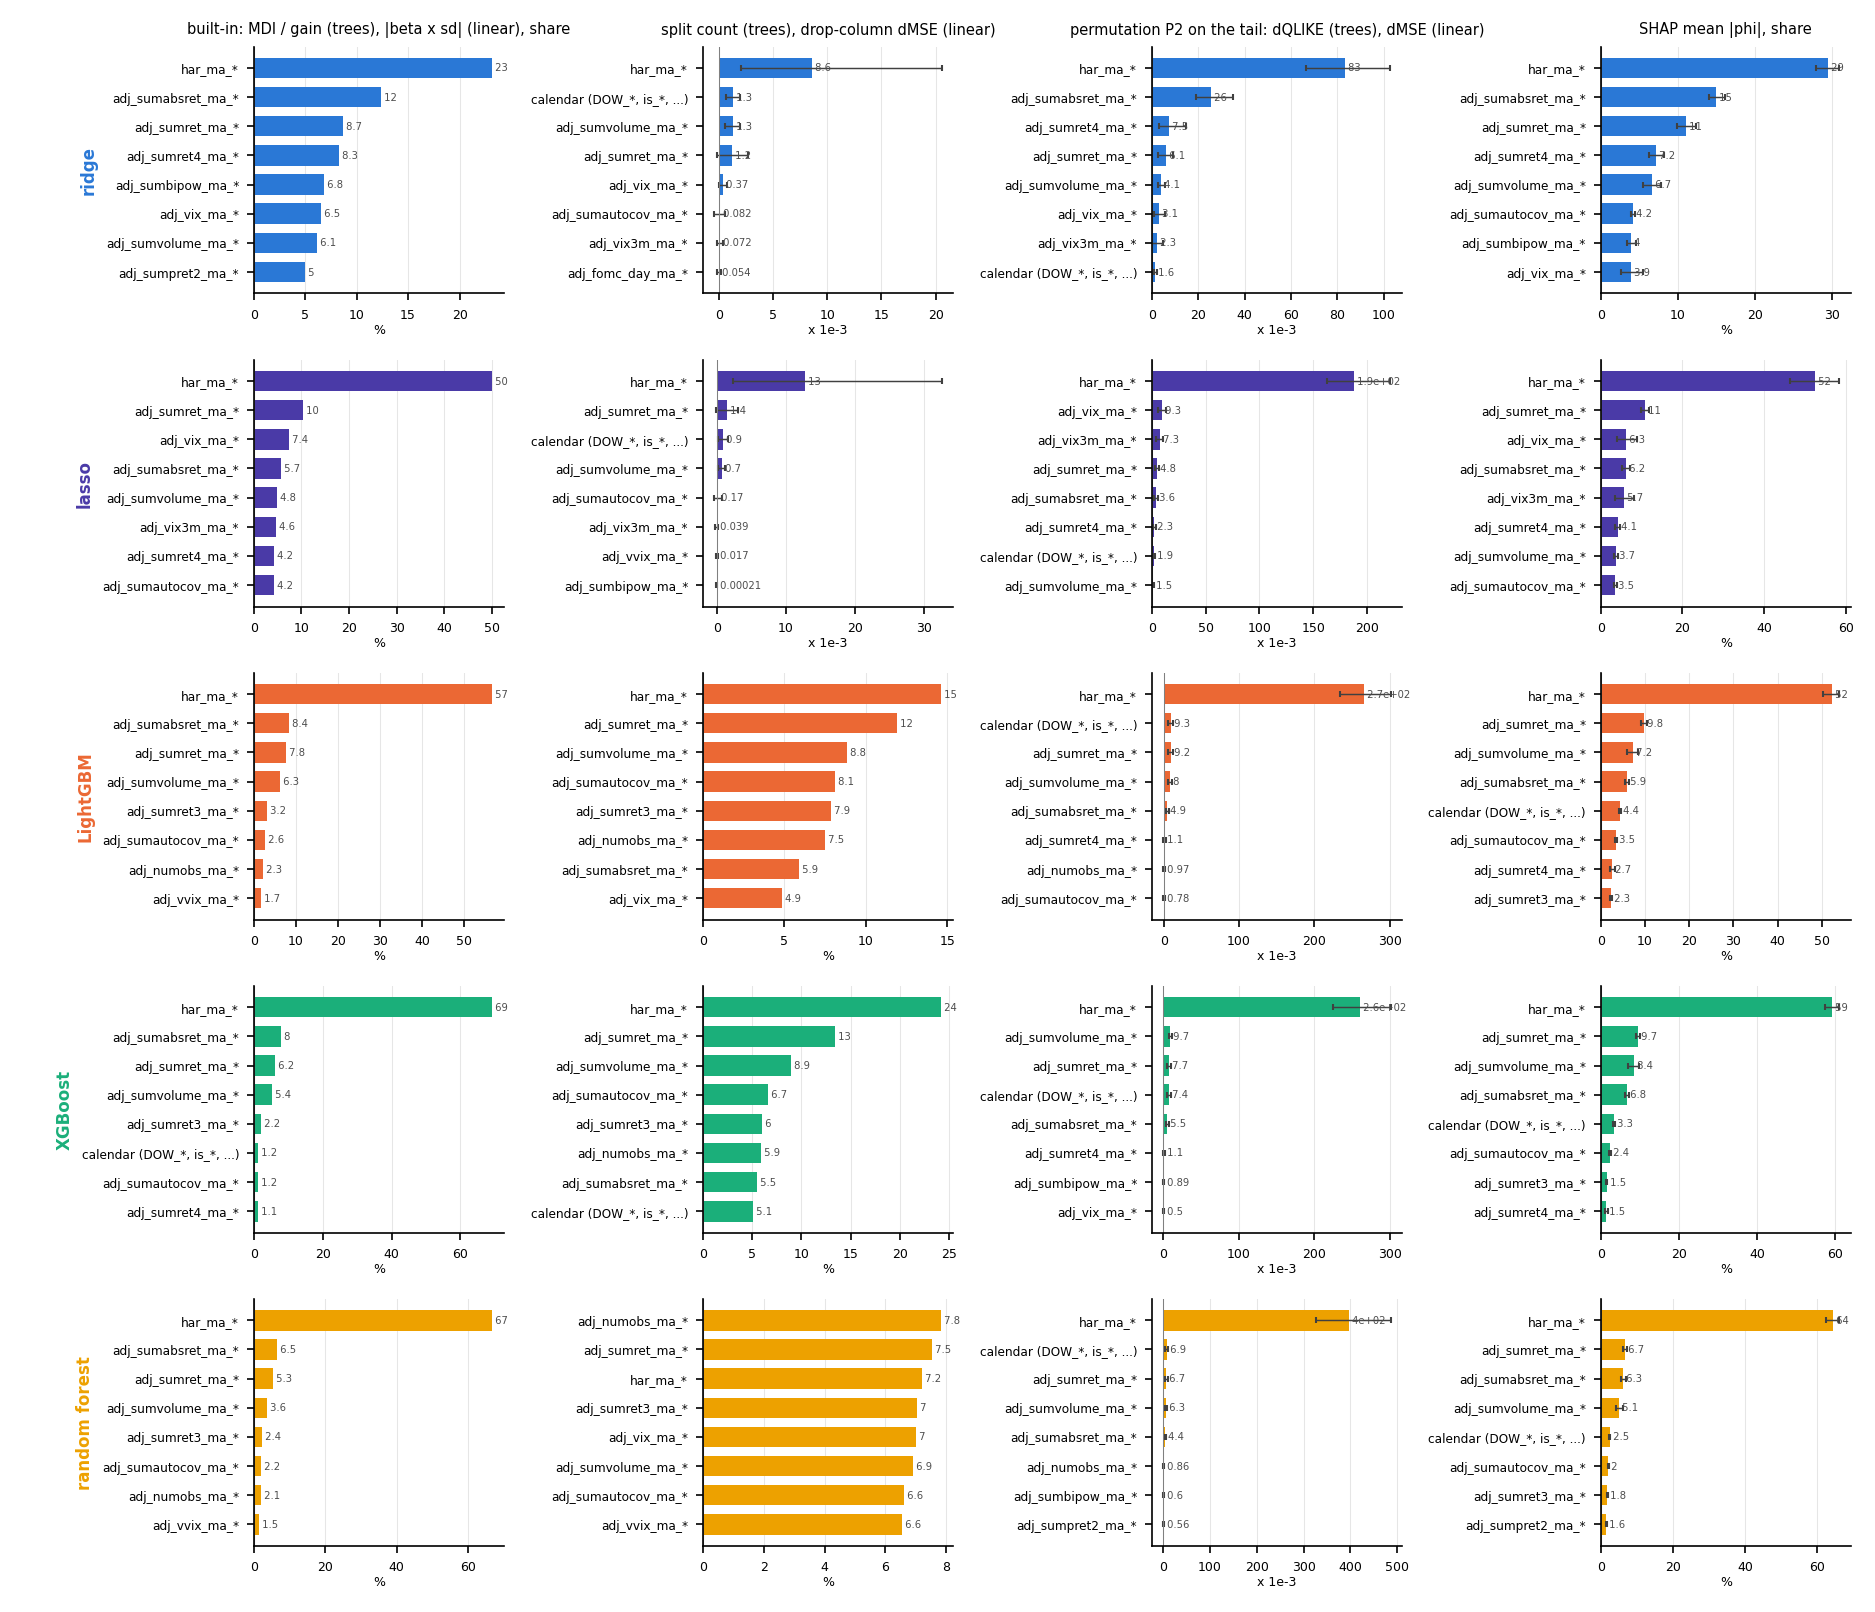
\includegraphics[width=\textwidth]{../results/feature_importance_1530_dedup/fig_ranked_live_feasible.png}
\caption{Live-feasible: ranked bars per measure (series level; top 8). Rows: models; columns: the built-in measure, split count (trees) / drop-column (linear), permutation P2 on the tail, SHAP. Bars with 95\% intervals over refits. Linear permutation / drop-column in $\Delta$MSE (see Section 6).}\end{figure}
\begin{table}[H]\centering\scriptsize
\caption{All-features design, series level: top three per model and measure.}
\begin{tabular}{llp{11.2cm}}\toprule
model & measure & top three\\\midrule
ridge & $|\beta\cdot sd|$ & \texttt{har\_ma\_*} 11\%; \texttt{adj\_sumabsret\_ma\_*} 5\%; \texttt{adj\_sumabsret\_vwstock\_ma\_*} 5\% \\
ridge & perm.\ P1, $\Delta$MSE & \texttt{har\_ma\_*} +69\%; \texttt{adj\_sumabsret\_vwstock\_ma\_*} +8\%; \texttt{adj\_sumabsret\_ma\_*} +7\% \\
ridge & perm.\ P2, $\Delta$MSE & \texttt{har\_ma\_*} +142\%; \texttt{adj\_sumabsret\_ma\_*} +22\%; \texttt{adj\_sumret4\_ma\_*} +18\% \\
ridge & perm.\ P2, $\Delta$QLIKE & \texttt{adj\_voldemand\_spx\_open\_only\_ma\_*} +59024\%; \texttt{adj\_stocktwits\_sentiment\_ma\_*} +4255\%; \texttt{adj\_sumret3\_ma\_*} +3480\% \\
ridge & drop-column, $\Delta$MSE & \texttt{har\_ma\_*} +17\%; \texttt{calendar} +2\%; \texttt{adj\_sumvolume\_ma\_*} +2\% \\
ridge & SHAP mean $|\phi|$ & \texttt{har\_ma\_*} 15\%; \texttt{adj\_sumabsret\_ma\_*} 6\%; \texttt{adj\_sumabsret\_vwstock\_ma\_*} 5\% \\
lasso & $|\beta\cdot sd|$ & \texttt{har\_ma\_*} 46\%; \texttt{adj\_sumabsret\_vwstock\_ma\_*} 10\%; \texttt{adj\_sumret\_ma\_*} 9\% \\
lasso & perm.\ P1, $\Delta$MSE & \texttt{har\_ma\_*} +156\%; \texttt{adj\_sumabsret\_vwstock\_ma\_*} +9\%; \texttt{adj\_sumret\_ma\_*} +7\% \\
lasso & perm.\ P2, $\Delta$MSE & \texttt{har\_ma\_*} +294\%; \texttt{adj\_sumabsret\_vwstock\_ma\_*} +17\%; \texttt{adj\_vix\_ma\_*} +15\% \\
lasso & perm.\ P2, $\Delta$QLIKE & \texttt{adj\_effspread\_vwstock\_ma\_*} +569\%; \texttt{har\_ma\_*} +259\%; \texttt{adj\_sumpret2\_vwstock\_ma\_*} +73\% \\
lasso & drop-column, $\Delta$MSE & \texttt{har\_ma\_*} +27\%; \texttt{adj\_sumret\_ma\_*} +2\%; \texttt{adj\_sumabsret\_vwstock\_ma\_*} +1\% \\
lasso & SHAP mean $|\phi|$ & \texttt{har\_ma\_*} 46\%; \texttt{adj\_sumabsret\_vwstock\_ma\_*} 10\%; \texttt{adj\_sumret\_ma\_*} 9\% \\
LightGBM & MDI / gain & \texttt{har\_ma\_*} 52\%; \texttt{adj\_sumabsret\_ma\_*} 6\%; \texttt{adj\_sumret\_ma\_*} 5\% \\
LightGBM & split count & \texttt{har\_ma\_*} 10\%; \texttt{adj\_sumret\_ma\_*} 6\%; \texttt{adj\_sumvolume\_ma\_*} 4\% \\
LightGBM & perm.\ P1, $\Delta$QLIKE & \texttt{har\_ma\_*} +97\%; \texttt{calendar} +5\%; \texttt{adj\_sumret\_ma\_*} +4\% \\
LightGBM & perm.\ P2, $\Delta$QLIKE & \texttt{har\_ma\_*} +200\%; \texttt{calendar} +6\%; \texttt{adj\_sumret\_ma\_*} +3\% \\
LightGBM & perm.\ P2, $\Delta$MSE & \texttt{har\_ma\_*} +204\%; \texttt{calendar} +4\%; \texttt{adj\_sumvolume\_ma\_*} +3\% \\
LightGBM & SHAP mean $|\phi|$ & \texttt{har\_ma\_*} 44\%; \texttt{adj\_sumret\_ma\_*} 6\%; \texttt{adj\_sumvolume\_ma\_*} 5\% \\
XGBoost & MDI / gain & \texttt{har\_ma\_*} 64\%; \texttt{adj\_sumabsret\_ma\_*} 7\%; \texttt{adj\_sumret\_ma\_*} 4\% \\
XGBoost & split count & \texttt{har\_ma\_*} 19\%; \texttt{adj\_sumret\_ma\_*} 8\%; \texttt{adj\_sumvolume\_ma\_*} 5\% \\
XGBoost & perm.\ P1, $\Delta$QLIKE & \texttt{har\_ma\_*} +95\%; \texttt{calendar} +4\%; \texttt{adj\_sumret\_ma\_*} +3\% \\
XGBoost & perm.\ P2, $\Delta$QLIKE & \texttt{har\_ma\_*} +187\%; \texttt{calendar} +5\%; \texttt{adj\_sumvolume\_ma\_*} +5\% \\
XGBoost & perm.\ P2, $\Delta$MSE & \texttt{har\_ma\_*} +193\%; \texttt{adj\_sumvolume\_ma\_*} +4\%; \texttt{calendar} +3\% \\
XGBoost & SHAP mean $|\phi|$ & \texttt{har\_ma\_*} 51\%; \texttt{adj\_sumret\_ma\_*} 7\%; \texttt{adj\_sumvolume\_ma\_*} 6\% \\
random forest & MDI / gain & \texttt{har\_ma\_*} 62\%; \texttt{adj\_sumabsret\_ma\_*} 5\%; \texttt{adj\_sumret\_ma\_*} 3\% \\
random forest & split count & \texttt{adj\_voldemand\_spx\_open\_and\_close\_ma\_*} 3\%; \texttt{har\_ma\_*} 3\%; \texttt{adj\_voldemand\_all\_open\_and\_close\_ma\_*} 3\% \\
random forest & perm.\ P1, $\Delta$QLIKE & \texttt{har\_ma\_*} +134\%; \texttt{calendar} +3\%; \texttt{adj\_sumabsret\_ma\_*} +2\% \\
random forest & perm.\ P2, $\Delta$QLIKE & \texttt{har\_ma\_*} +283\%; \texttt{calendar} +4\%; \texttt{adj\_sumabsret\_ma\_*} +3\% \\
random forest & perm.\ P2, $\Delta$MSE & \texttt{har\_ma\_*} +246\%; \texttt{calendar} +2\%; \texttt{adj\_sumvolume\_ma\_*} +1\% \\
random forest & SHAP mean $|\phi|$ & \texttt{har\_ma\_*} 58\%; \texttt{adj\_sumabsret\_ma\_*} 5\%; \texttt{adj\_sumret\_ma\_*} 4\% \\
\bottomrule\end{tabular}\end{table}
\begin{figure}[H]\centering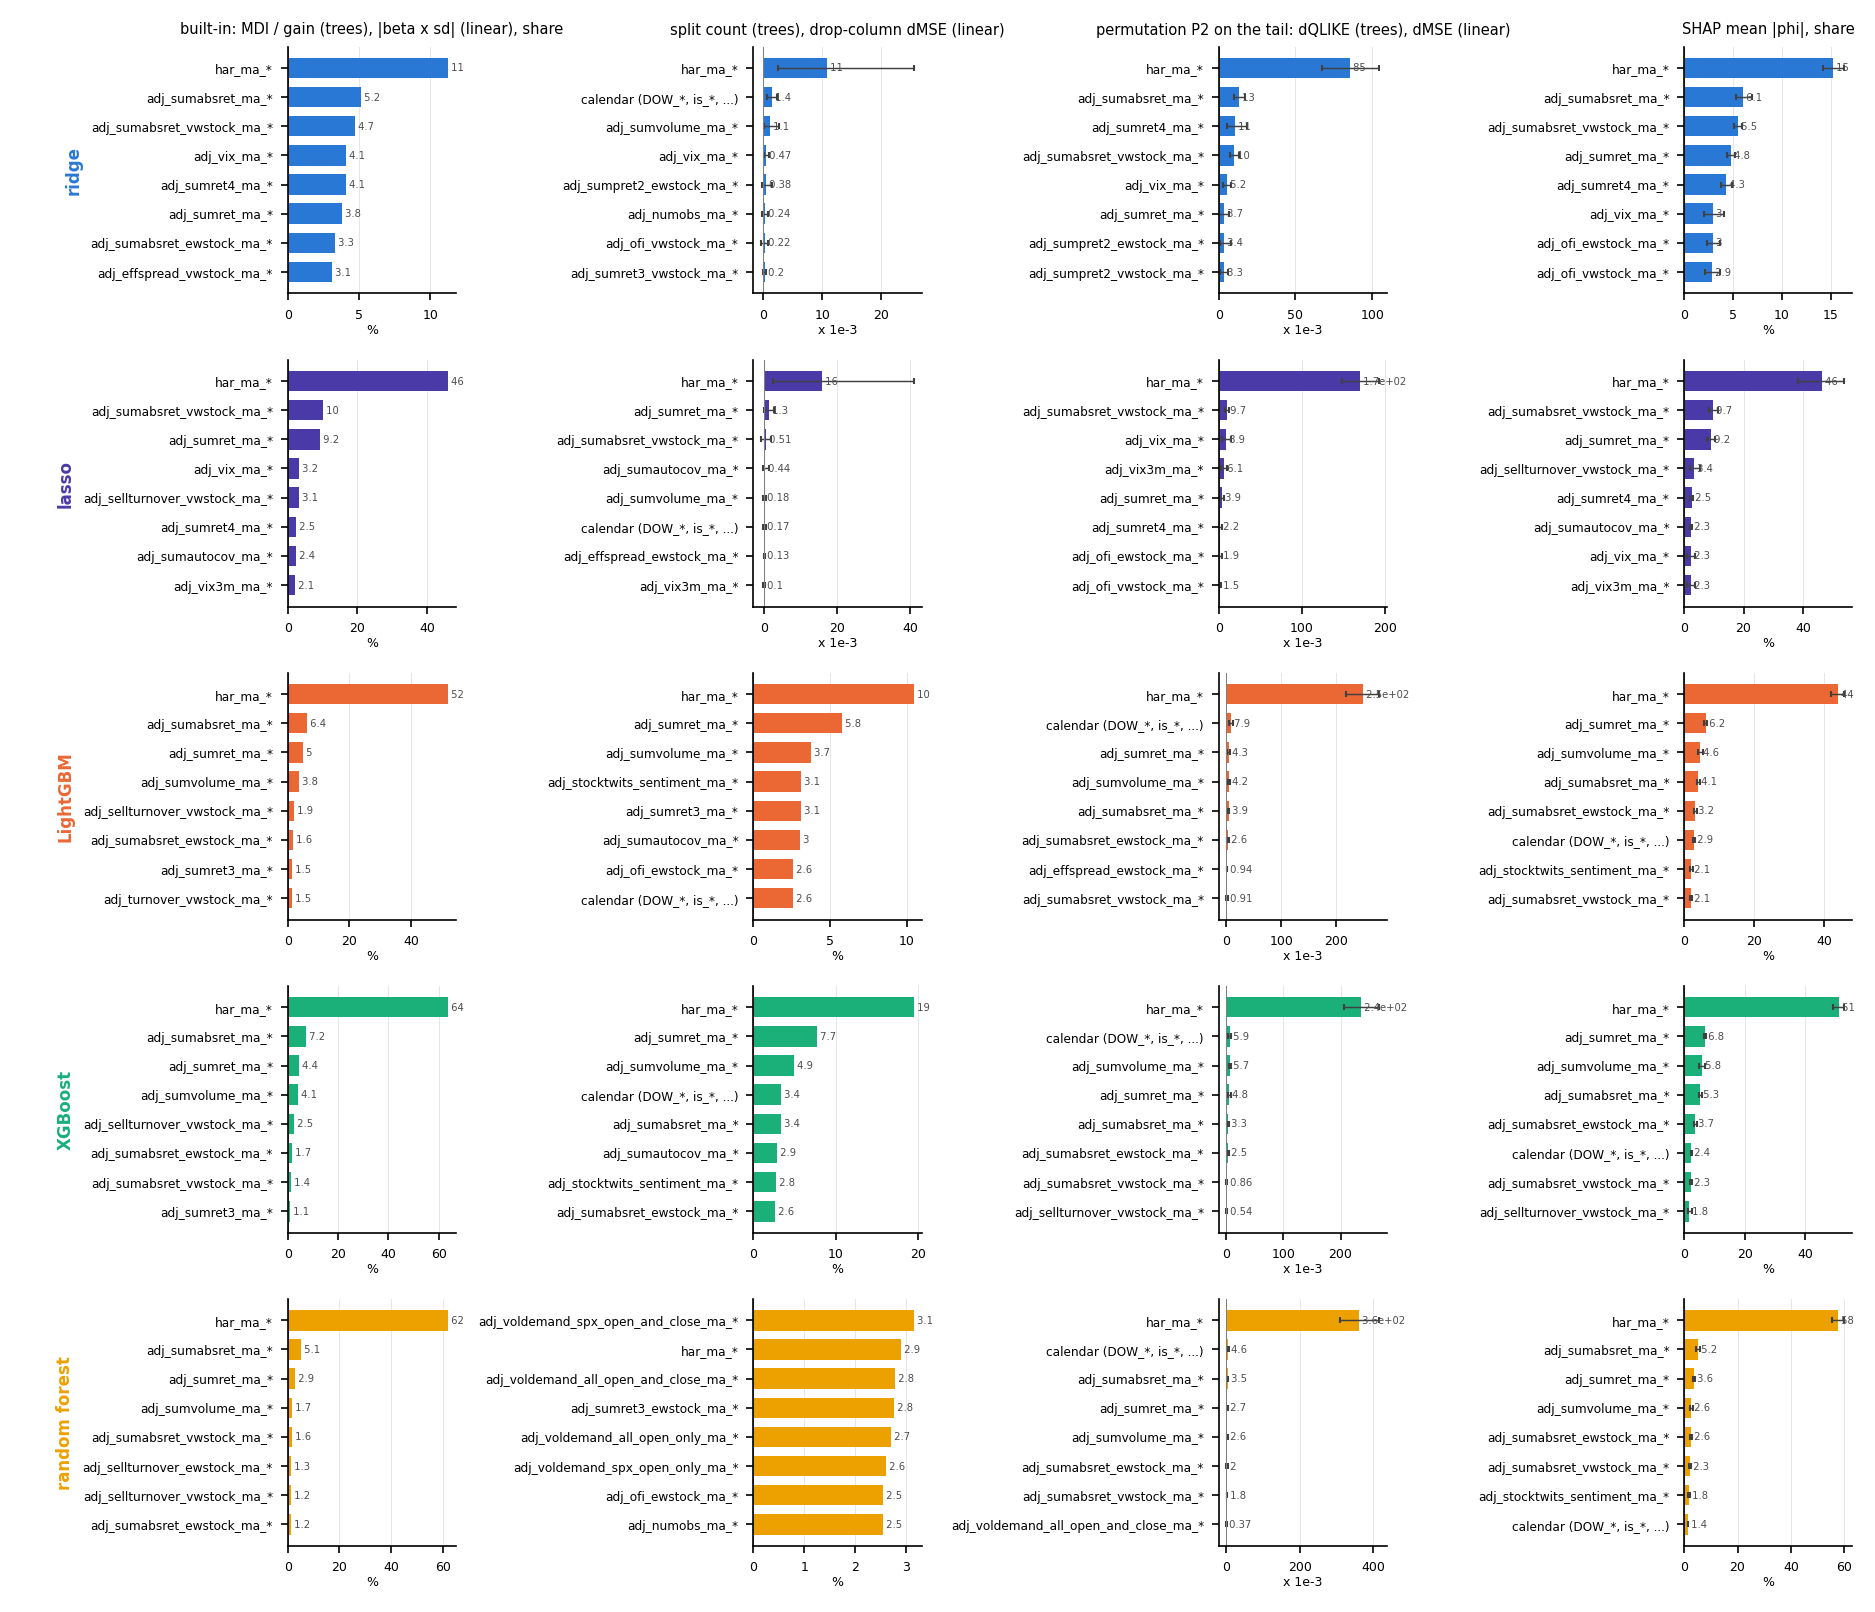
\includegraphics[width=\textwidth]{../results/feature_importance_1530_dedup/fig_ranked_all_features.png}
\caption{All features: ranked bars per measure (series level; top 8).}\end{figure}

\section*{3. Ranking agreement}
\begin{table}[H]\centering\scriptsize
\caption{Within a tree model: Spearman between measures (series / column level).}
\begin{tabular}{lllrrrrrr}\toprule
bucket & level & model & MDI$\sim$split & MDI$\sim$SHAP & MDI$\sim$P2 & SHAP$\sim$P2 & P1$\sim$P2 & P2 QL$\sim$MSE\\\midrule
live-feasible & series & LightGBM & 0.95 & 0.89 & 0.59 & 0.71 & 0.82 & 0.91 \\
live-feasible & series & XGBoost & 0.90 & 0.95 & 0.69 & 0.80 & 0.86 & 0.92 \\
live-feasible & series & random forest & 0.80 & 0.82 & 0.62 & 0.77 & 0.86 & 0.88 \\
live-feasible & column & LightGBM & 0.99 & 0.97 & 0.19 & 0.22 & 0.60 & 0.51 \\
live-feasible & column & XGBoost & 0.99 & 0.97 & 0.46 & 0.45 & 0.62 & 0.62 \\
live-feasible & column & random forest & 0.97 & 0.98 & 0.21 & 0.21 & 0.67 & 0.62 \\
all features & series & LightGBM & 0.87 & 0.87 & 0.21 & 0.27 & 0.69 & 0.72 \\
all features & series & XGBoost & 0.87 & 0.88 & 0.52 & 0.56 & 0.78 & 0.58 \\
all features & series & random forest & 0.55 & 0.86 & 0.17 & 0.31 & 0.68 & 0.68 \\
all features & column & LightGBM & 0.99 & 0.97 & 0.06 & 0.05 & 0.53 & 0.60 \\
all features & column & XGBoost & 0.99 & 0.97 & 0.26 & 0.25 & 0.55 & 0.47 \\
all features & column & random forest & 0.98 & 0.98 & 0.03 & 0.03 & 0.45 & 0.51 \\
\bottomrule\end{tabular}\end{table}
\begin{table}[H]\centering\scriptsize
\caption{Within a linear model: Spearman between measures.}
\begin{tabular}{lllrrrrrr}\toprule
bucket & level & model & $|\beta sd|\sim$SHAP & $|\beta sd|\sim$P2 & SHAP$\sim$P2 & P1$\sim$P2 & P2$\sim$drop & P2 QL$\sim$MSE\\\midrule
live-feasible & series & ridge & 0.95 & 0.87 & 0.90 & 0.87 & 0.45 & 0.72 \\
live-feasible & series & lasso & 0.96 & 0.93 & 0.93 & 0.78 & 0.36 & 0.95 \\
live-feasible & column & ridge & 0.98 & 0.53 & 0.51 & 0.65 & 0.42 & 0.15 \\
live-feasible & column & lasso & 0.98 & 0.51 & 0.46 & 0.58 & 0.12 & 0.75 \\
all features & series & ridge & 0.83 & 0.59 & 0.73 & 0.77 & 0.38 & -0.05 \\
all features & series & lasso & 0.95 & 0.88 & 0.86 & 0.82 & 0.13 & 0.95 \\
all features & column & ridge & 0.99 & 0.42 & 0.42 & 0.58 & 0.16 & 0.09 \\
all features & column & lasso & 0.99 & 0.40 & 0.38 & 0.65 & 0.13 & 0.78 \\
\bottomrule\end{tabular}\end{table}
\begin{table}[H]\centering\scriptsize
\caption{Across models, same measure: range of Spearman over tree--tree pairs, tree--linear pairs, and ridge--lasso.}
\begin{tabular}{llrrrrrrrrr}\toprule
bucket & level & \multicolumn{3}{c}{SHAP} & \multicolumn{3}{c}{perm P2 $\Delta$QLIKE} & \multicolumn{3}{c}{perm P2 $\Delta$MSE}\\ & & tree & tree--lin & r--l & tree & tree--lin & r--l & tree & tree--lin & r--l\\\midrule
live-feasible & series & 0.89--0.95 & 0.56--0.76 & 0.84 & 0.74--0.91 & 0.33--0.61 & 0.62 & 0.67--0.83 & 0.50--0.85 & 0.88 \\
live-feasible & column & 0.96--0.98 & 0.69--0.83 & 0.80 & 0.33--0.47 & 0.08--0.29 & 0.19 & 0.12--0.41 & 0.17--0.31 & 0.39 \\
all features & series & 0.83--0.89 & 0.32--0.49 & 0.86 & 0.39--0.61 & -0.26--0.37 & -0.10 & 0.49--0.58 & 0.01--0.49 & 0.69 \\
all features & column & 0.95--0.97 & 0.68--0.88 & 0.78 & 0.17--0.27 & -0.13--0.10 & 0.09 & 0.23--0.26 & -0.00--0.07 & 0.43 \\
\bottomrule\end{tabular}\end{table}
\begin{figure}[H]\centering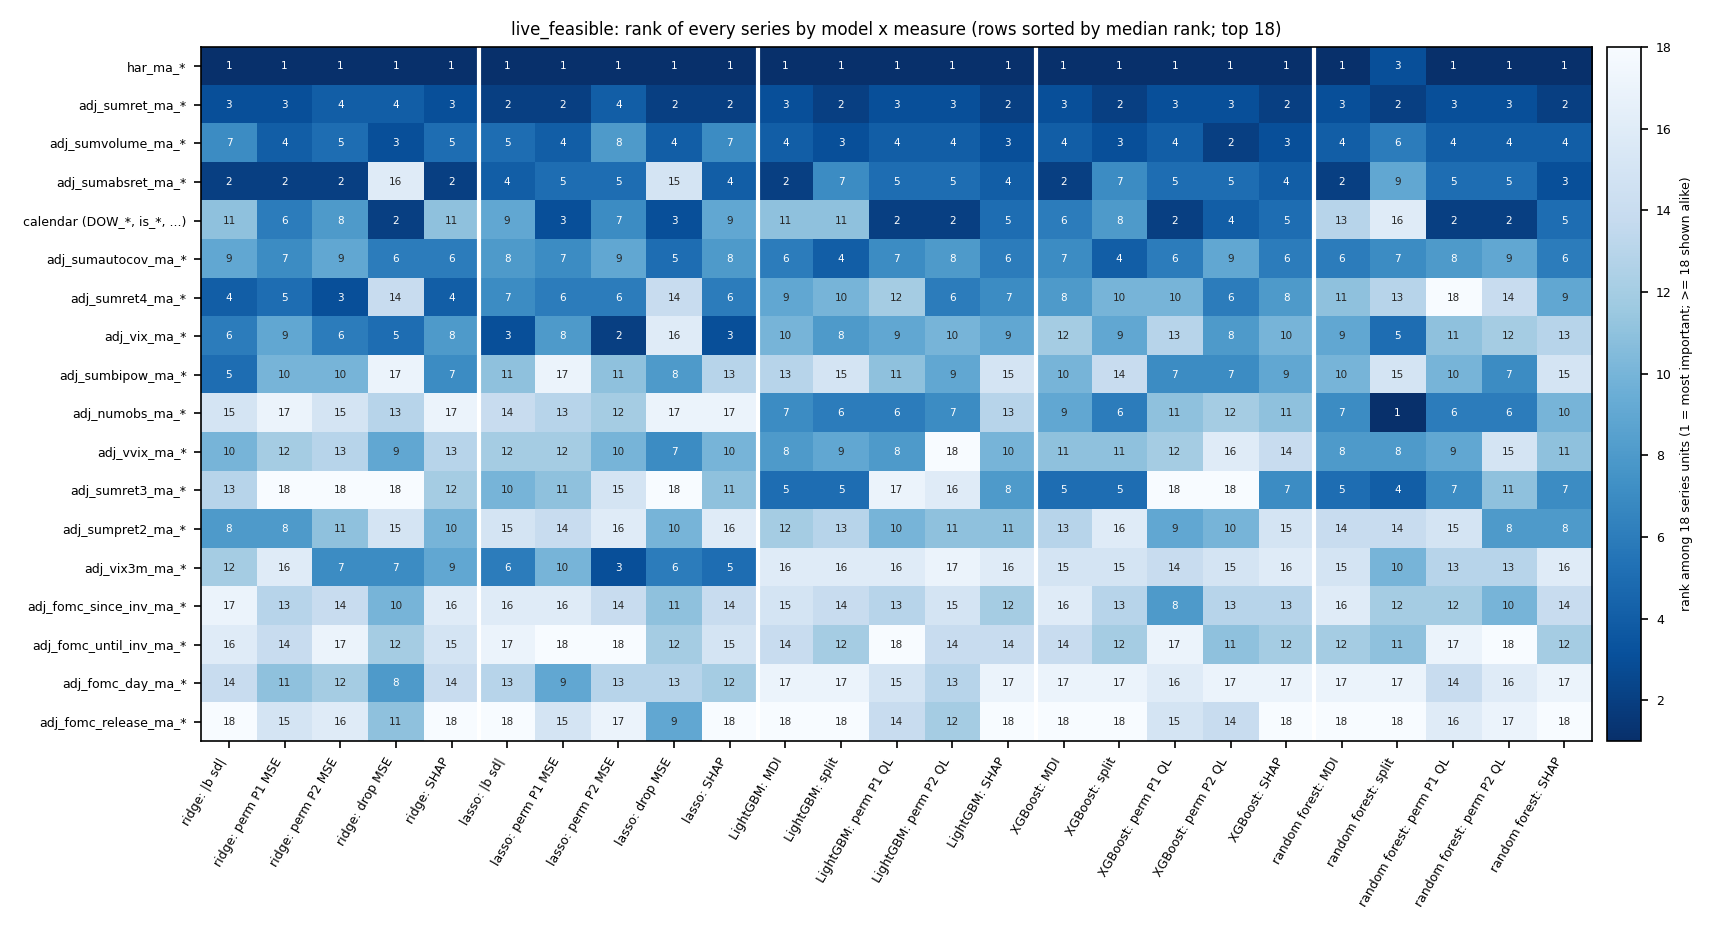
\includegraphics[width=0.95\textwidth]{../results/feature_importance_1530_dedup/fig_rank_heatmap_live_feasible_series.png}
\caption{Live-feasible: rank of every series under every model $\times$ measure (1 = most important).}\end{figure}
\begin{figure}[H]\centering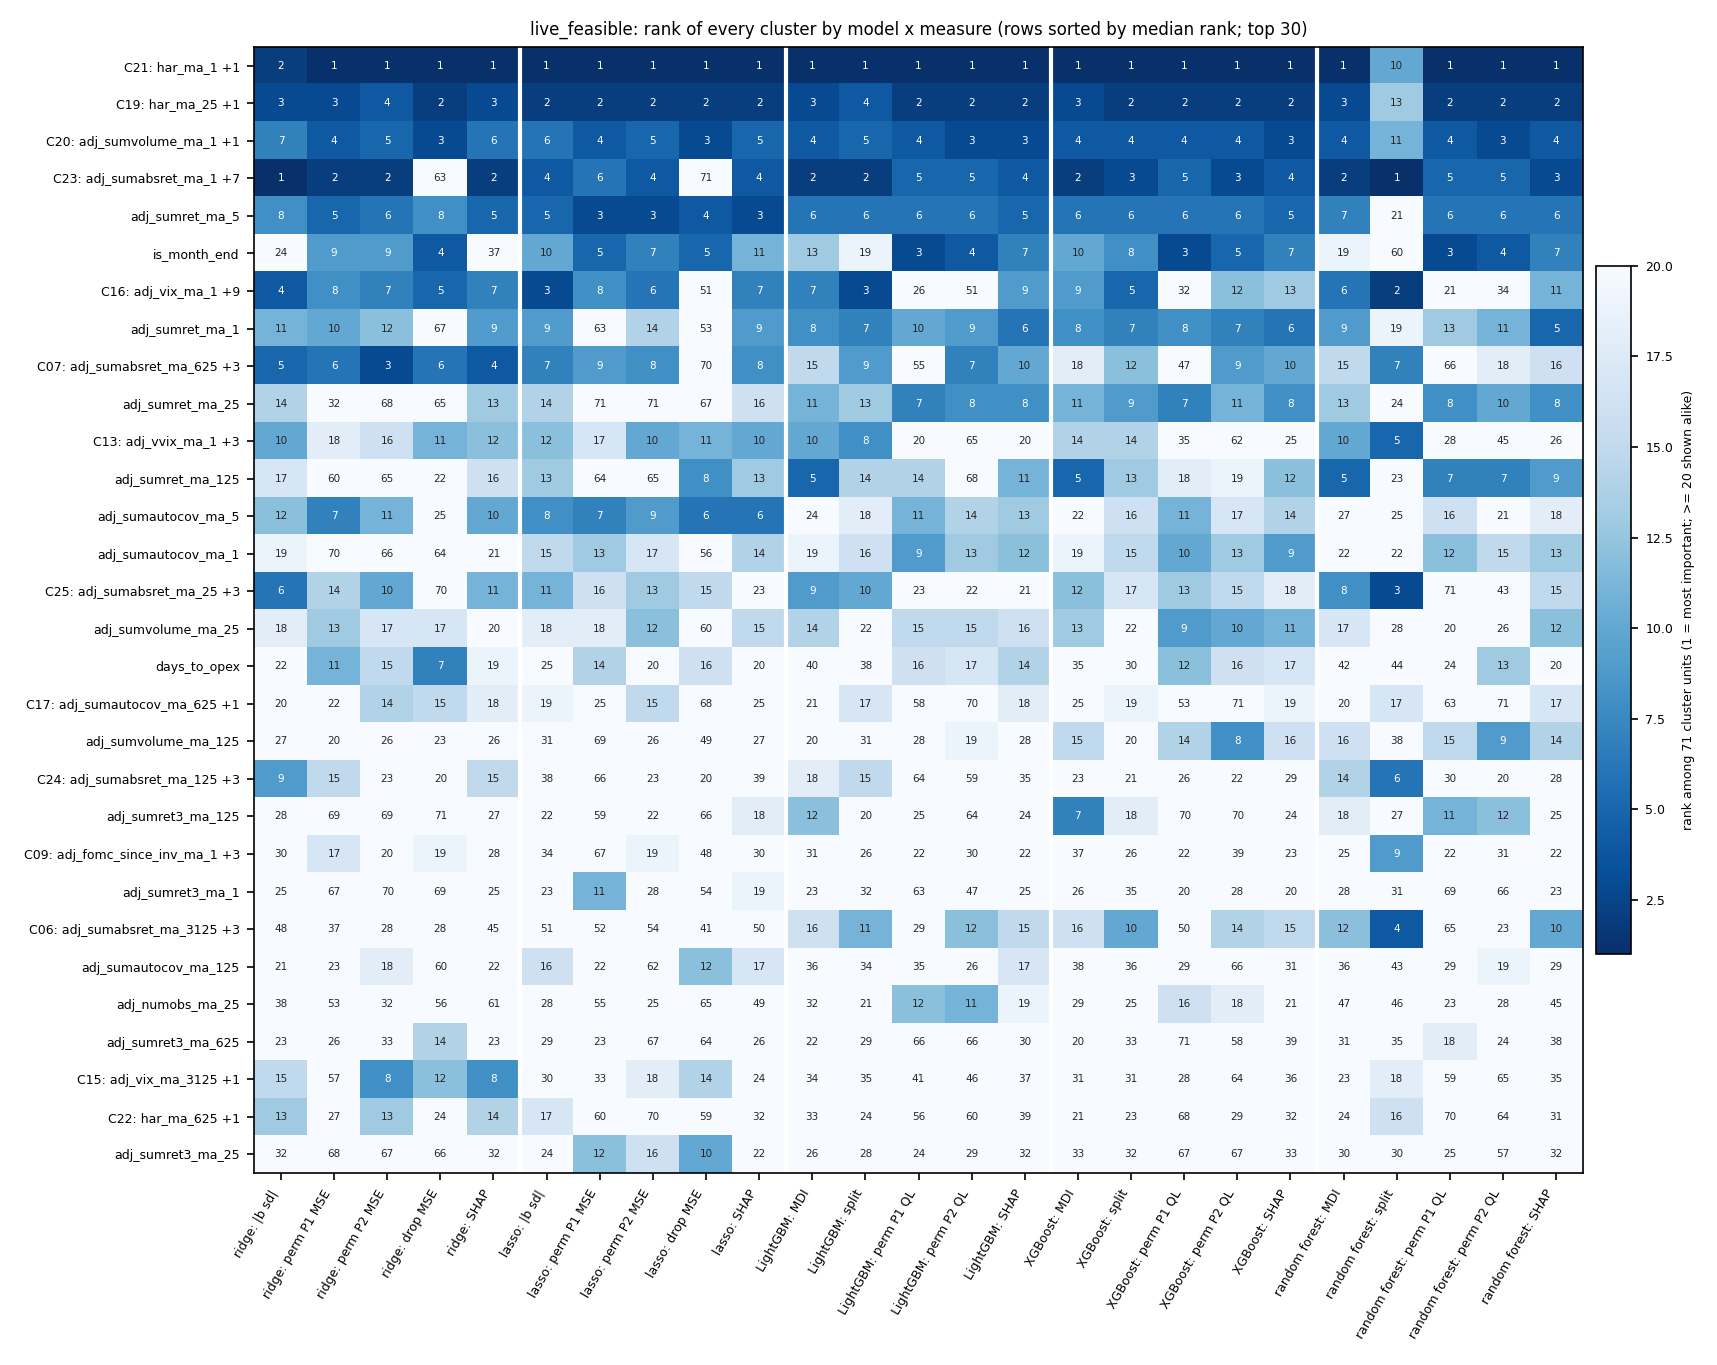
\includegraphics[width=0.95\textwidth]{../results/feature_importance_1530_dedup/fig_rank_heatmap_live_feasible_cluster.png}
\caption{Live-feasible: the same at the cluster level (clusters of $|$corr$|\ge0.8$; a singleton is its column).}\end{figure}
\begin{figure}[H]\centering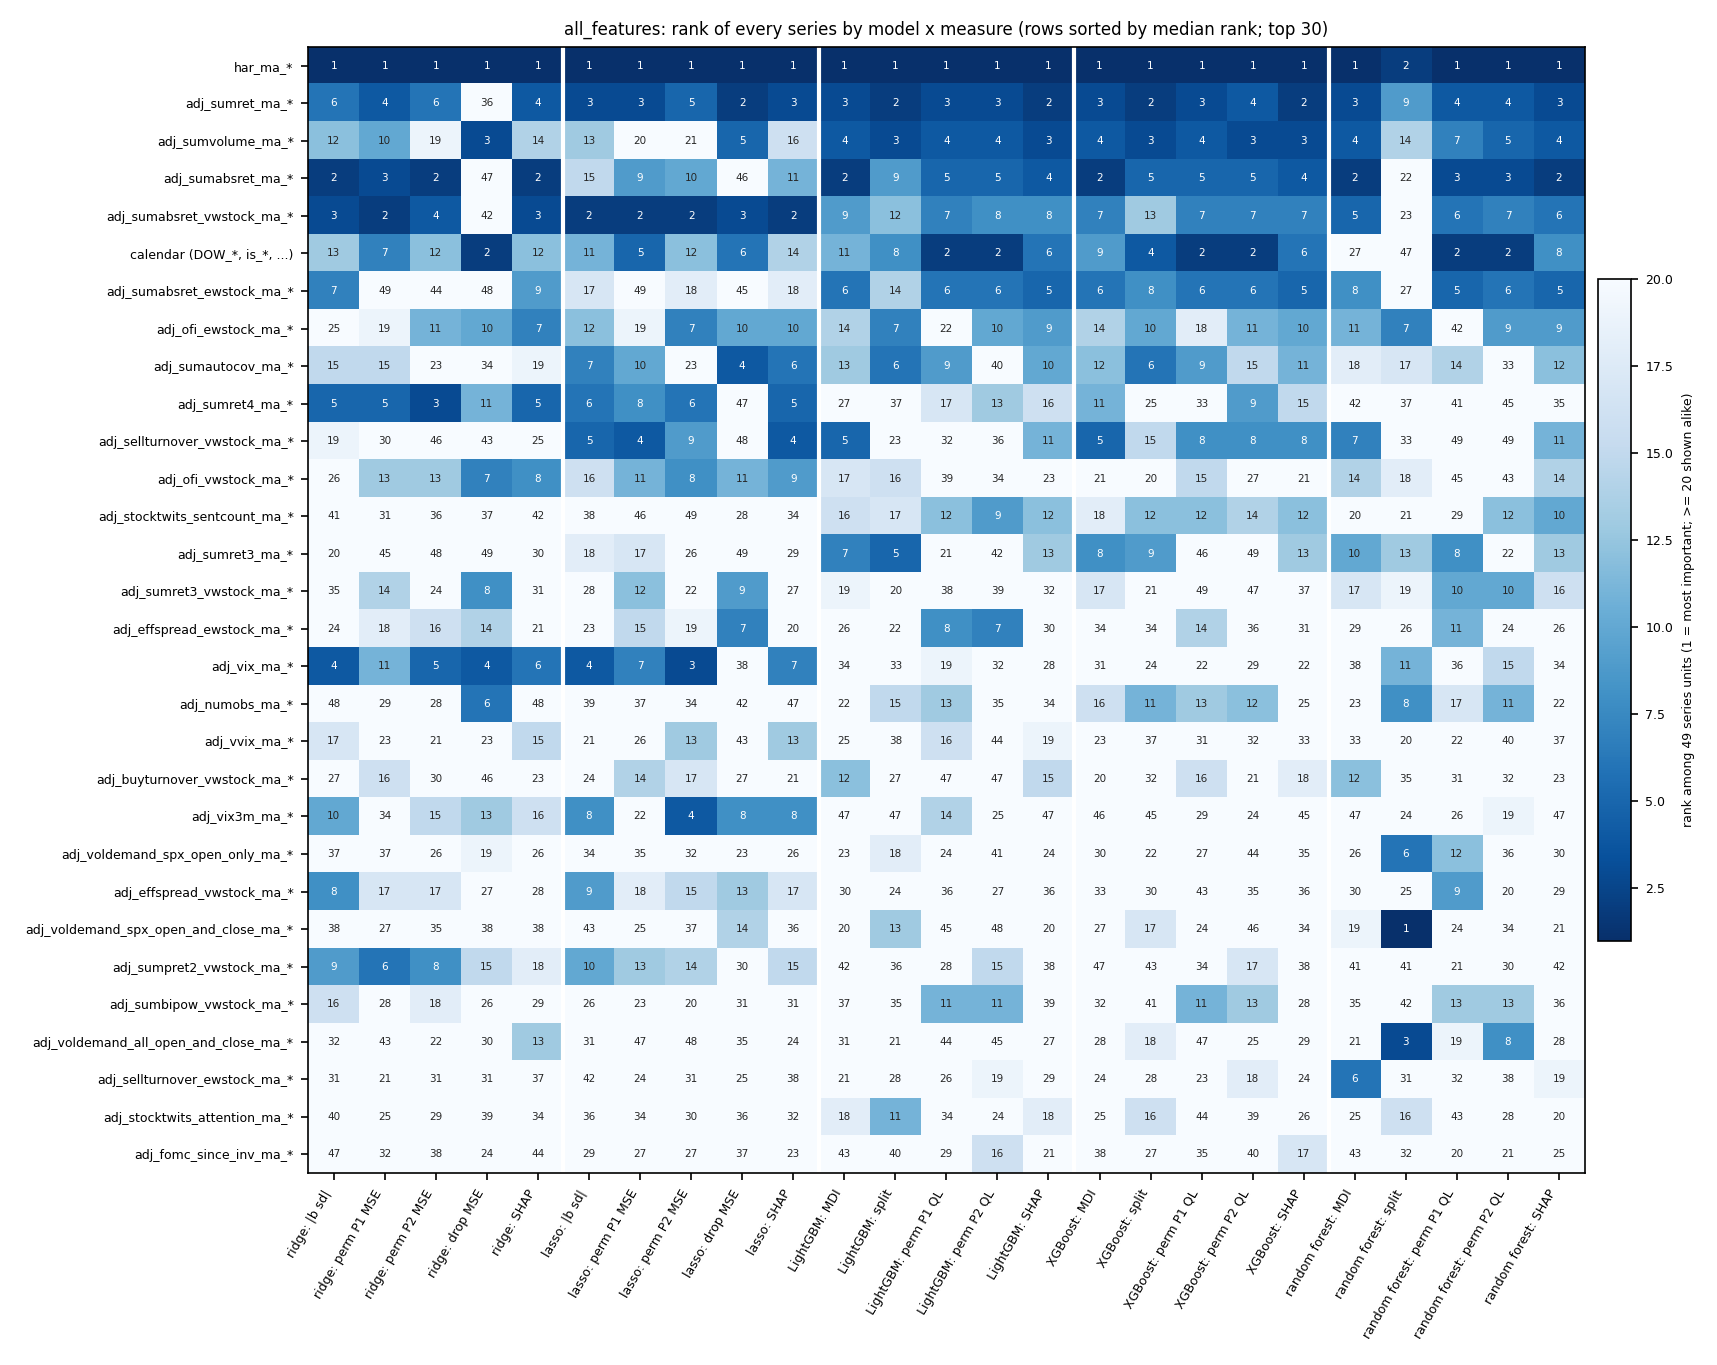
\includegraphics[width=0.95\textwidth]{../results/feature_importance_1530_dedup/fig_rank_heatmap_all_features_series.png}
\caption{All features: rank of every series under every model $\times$ measure.}\end{figure}

\section*{4. Stability over refits and regimes}
\begin{table}[H]\centering\scriptsize
\caption{Top-5 stability (series level): share of the 147 refits in which \texttt{har\_ma\_*} is in the refit's top 5; number of series in the top 5 in at least half the refits; number ever in the top 5. Measures: built-in (MDI or $|\beta sd|$), permutation P2 ($\Delta$QLIKE trees, $\Delta$MSE linear), SHAP.}
\begin{tabular}{llrrrrrrrrr}\toprule
bucket & model & \multicolumn{3}{c}{built-in} & \multicolumn{3}{c}{perm P2} & \multicolumn{3}{c}{SHAP}\\ & & har & $\ge$50\% & ever & har & $\ge$50\% & ever & har & $\ge$50\% & ever\\\midrule
live-feasible & ridge & 100\% & 5 & 10 & 99\% & 4 & 17 & 100\% & 5 & 15 \\
live-feasible & lasso & 100\% & 3 & 9 & 100\% & 4 & 15 & 100\% & 3 & 10 \\
live-feasible & LightGBM & 100\% & 5 & 6 & 99\% & 5 & 18 & 100\% & 5 & 16 \\
live-feasible & XGBoost & 100\% & 5 & 9 & 99\% & 4 & 17 & 100\% & 5 & 12 \\
live-feasible & random forest & 100\% & 5 & 7 & 100\% & 3 & 18 & 100\% & 4 & 14 \\
all features & ridge & 100\% & 5 & 11 & 98\% & 3 & 44 & 99\% & 3 & 27 \\
all features & lasso & 100\% & 4 & 12 & 100\% & 3 & 30 & 100\% & 3 & 24 \\
all features & LightGBM & 100\% & 5 & 10 & 99\% & 2 & 47 & 100\% & 4 & 28 \\
all features & XGBoost & 100\% & 5 & 10 & 99\% & 3 & 47 & 100\% & 4 & 15 \\
all features & random forest & 100\% & 4 & 13 & 99\% & 1 & 48 & 100\% & 5 & 29 \\
\bottomrule\end{tabular}\end{table}
\begin{table}[H]\centering\scriptsize
\caption{Regimes: Spearman between the ranking within a stratum and the full-sample ranking (series level): median (minimum) over the calendar years (2018: 13, 2019: 26, 2020: 25, 2021: 25, 2022: 25, 2023: 25, 2024: 8 refits) and over the causal VIX terciles (VIX at 15:30 against the 1/3, 2/3 quantiles of the previous 2000 sessions' 15:30 VIX: low 28, mid 38, high 81 refits); years in which the full-sample leader also leads.}
\begin{tabular}{llrrrrrrrrr}\toprule
bucket & model & \multicolumn{3}{c}{built-in} & \multicolumn{3}{c}{perm P2} & \multicolumn{3}{c}{SHAP}\\ & & year & VIX & lead & year & VIX & lead & year & VIX & lead\\\midrule
live-feasible & ridge & 0.98 (0.91) & 1.00 (0.99) & 7/7 & 0.84 (0.74) & 0.93 (0.81) & 7/7 & 0.93 (0.81) & 0.98 (0.93) & 7/7 \\
live-feasible & lasso & 0.81 (0.61) & 0.99 (0.99) & 7/7 & 0.80 (0.32) & 0.89 (0.73) & 7/7 & 0.83 (0.64) & 0.98 (0.98) & 7/7 \\
live-feasible & LightGBM & 0.99 (0.96) & 0.99 (0.99) & 7/7 & 0.73 (0.39) & 0.84 (0.74) & 7/7 & 0.96 (0.92) & 0.97 (0.97) & 7/7 \\
live-feasible & XGBoost & 0.98 (0.95) & 0.99 (0.98) & 7/7 & 0.78 (0.44) & 0.89 (0.81) & 7/7 & 0.96 (0.83) & 0.99 (0.98) & 7/7 \\
live-feasible & random forest & 0.96 (0.92) & 0.99 (0.99) & 7/7 & 0.73 (0.24) & 0.81 (0.64) & 7/7 & 0.96 (0.80) & 0.98 (0.98) & 7/7 \\
all features & ridge & 0.93 (0.84) & 0.99 (0.95) & 7/7 & 0.67 (0.50) & 0.78 (0.60) & 7/7 & 0.76 (0.54) & 0.92 (0.83) & 7/7 \\
all features & lasso & 0.60 (0.47) & 0.99 (0.84) & 7/7 & 0.39 (0.15) & 0.72 (0.31) & 7/7 & 0.64 (0.42) & 0.97 (0.83) & 7/7 \\
all features & LightGBM & 0.94 (0.87) & 0.99 (0.98) & 7/7 & 0.60 (0.31) & 0.66 (0.61) & 7/7 & 0.83 (0.73) & 0.93 (0.93) & 7/7 \\
all features & XGBoost & 0.94 (0.88) & 0.99 (0.98) & 7/7 & 0.57 (0.10) & 0.65 (0.51) & 7/7 & 0.87 (0.66) & 0.93 (0.92) & 7/7 \\
all features & random forest & 0.98 (0.94) & 0.99 (0.98) & 7/7 & 0.49 (0.32) & 0.60 (0.31) & 7/7 & 0.90 (0.77) & 0.97 (0.96) & 7/7 \\
\bottomrule\end{tabular}\end{table}
\begin{figure}[H]\centering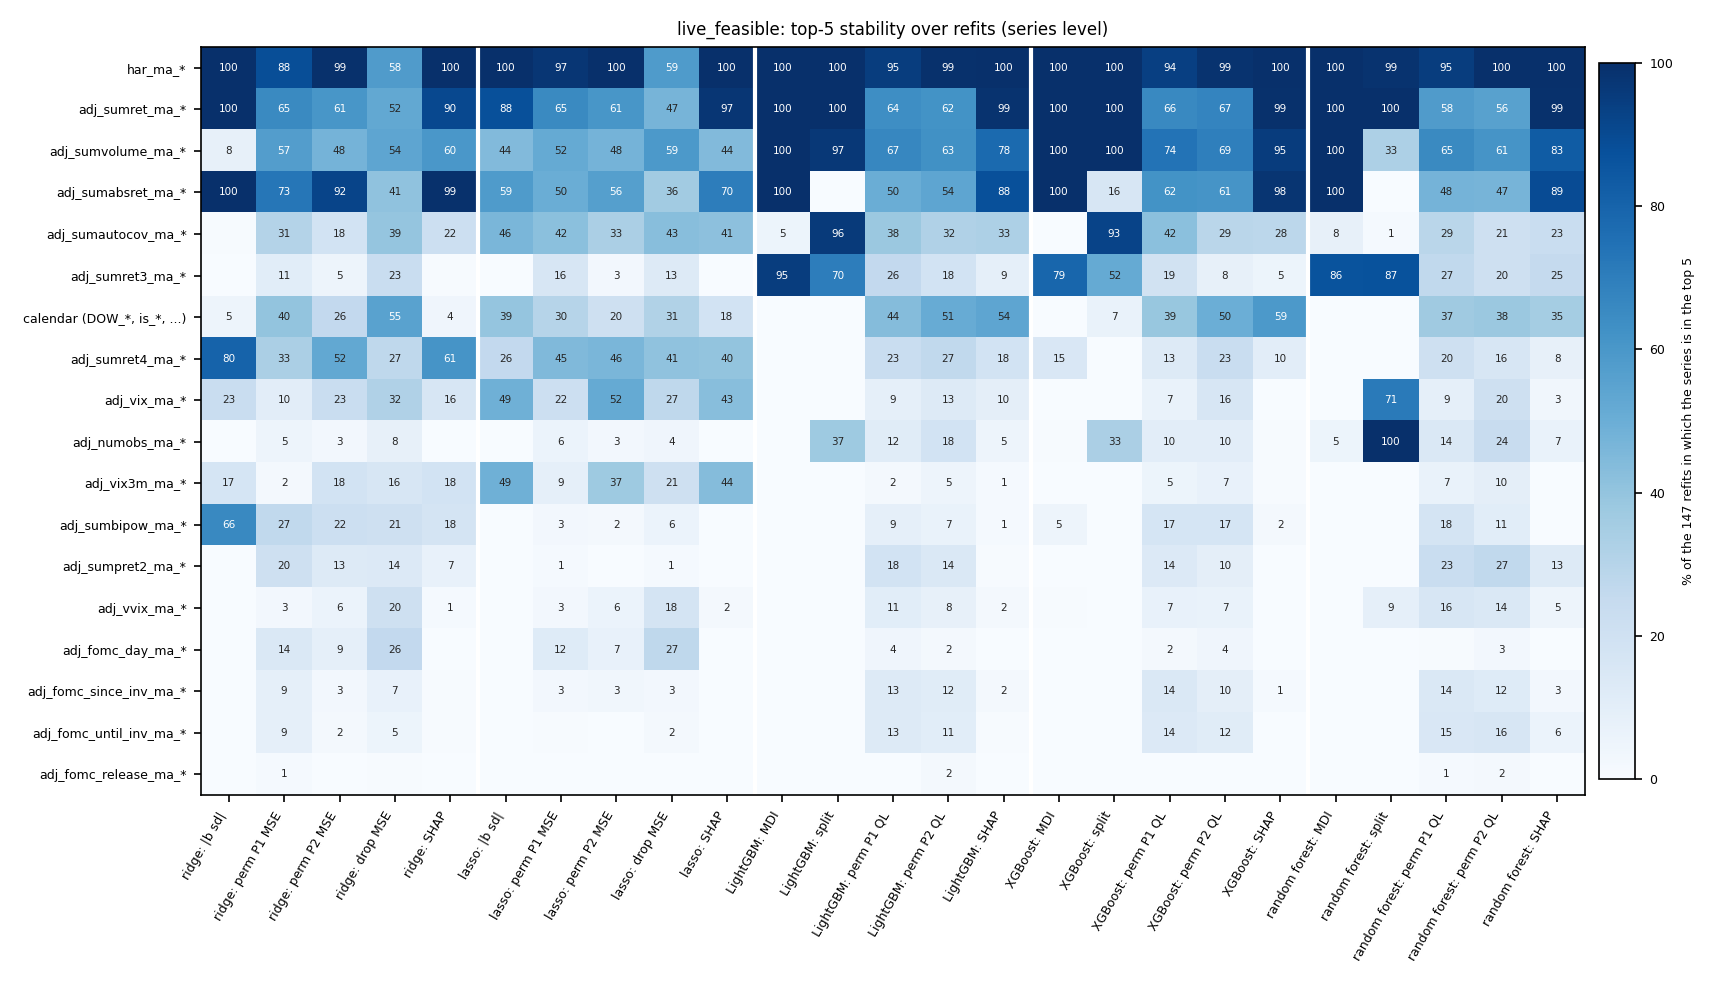
\includegraphics[width=0.95\textwidth]{../results/feature_importance_1530_dedup/fig_top5_stability_live_feasible.png}
\caption{Live-feasible: \% of refits in which each series is in the top 5, per model $\times$ measure.}\end{figure}

\section*{5. Correlated inputs: the dilution caveat}
\begin{table}[H]\centering\scriptsize
\caption{Joint permutation of a cluster against the sum of its columns permuted one at a time (P2, $\Delta$MSE in the fit space $\times10^{3}$, joint / sum; squared error so the linear columns are not dominated by single tails), for the four clusters with the largest joint effect in LightGBM. Joint $>$ sum: the columns substitute for one another and one-at-a-time permutation understates the group (dilution). Joint $<$ sum: offsetting weights (permuting one column breaks an offset its partner carries).}
\begin{tabular}{llp{5.2cm}rrrrr}\toprule
bucket & cluster & members & ridge & lasso & LightGBM & XGBoost & forest\\\midrule
live-feasible & C21 & \texttt{har\_ma\_1, har\_ma\_5} (2; $|r|\ge$0.89) & 33.5 / 18.9 & 100.0 / 64.0 & 92.3 / 46.6 & 91.4 / 51.6 & 147.4 / 80.9 \\
live-feasible & C19 & \texttt{har\_ma\_25, har\_ma\_125} (2; $|r|\ge$0.83) & 13.4 / 8.6 & 21.7 / 14.4 & 6.4 / 4.1 & 7.5 / 5.2 & 4.8 / 3.6 \\
live-feasible & C20 & \texttt{adj\_sumvolume\_ma\_1, adj\_sumvolume\_ma\_5} (2; $|r|\ge$0.89) & 3.6 / 2.1 & 2.2 / 1.4 & 2.2 / 1.0 & 3.1 / 2.1 & 1.5 / 0.9 \\
live-feasible & C23 & \texttt{adj\_sumabsret\_ma\_1, adj\_sumabsret\_ma\_5, adj\_sumret4\_ma\_1, adj\_sumret4\_ma\_5 +4} (8; $|r|\ge$0.82) & 29.3 / 7.7 & 2.3 / 4.7 & 0.8 / -2.4 & 5.6 / 1.0 & 2.4 / -0.1 \\
all features & C49 & \texttt{har\_ma\_1, har\_ma\_5} (2; $|r|\ge$0.89) & 33.2 / 18.3 & 85.7 / 50.0 & 86.9 / 45.6 & 80.2 / 45.3 & 139.1 / 75.9 \\
all features & C46 & \texttt{har\_ma\_25, har\_ma\_125} (2; $|r|\ge$0.83) & 13.3 / 7.3 & 20.0 / 11.9 & 6.4 / 4.2 & 7.0 / 4.6 & 3.1 / 2.2 \\
all features & C51 & \texttt{adj\_sumabsret\_ma\_1, adj\_sumabsret\_ma\_5, adj\_sumret4\_ma\_1, adj\_sumret4\_ma\_5 +4} (8; $|r|\ge$0.82) & 7.2 / 3.6 & 0.5 / 2.6 & 1.7 / -0.6 & 2.1 / -0.8 & 0.7 / -0.8 \\
all features & C50 & \texttt{adj\_sumabsret\_ewstock\_ma\_1, adj\_sumabsret\_ewstock\_ma\_5, adj\_sumabsret\_vwstock\_ma\_1, adj\_sumabsret\_vwstock\_ma\_5} (4; $|r|\ge$0.85) & 15.5 / 3.9 & 8.7 / 7.0 & 1.4 / 0.6 & 0.3 / -0.4 & 1.4 / 0.4 \\
\bottomrule\end{tabular}\end{table}

\section*{6. Linear models: QLIKE permutation is dominated by single tails}
The linear forecasts are unbounded: moving an extreme input (a crash day's 4th-power or absolute return) onto another row can push the fit-space forecast through zero, and QLIKE of $\hat y^2\times$ baseline explodes. Every permutation / drop-column table therefore carries the median refit and the largest single-refit share of the sum, and the linear figures and cross-model comparisons use the squared-error versions. Trees cannot extrapolate beyond the training range of the target, so their QLIKE changes are well behaved.
\begin{table}[H]\centering\scriptsize
\caption{The top linear QLIKE entries: mean [95\% interval], median refit, share of the sum carried by one refit.}
\begin{tabular}{lllllrr}\toprule
bucket & model & measure & top series & mean [interval] & median & one refit\\\midrule
live-feasible & ridge & perm.\ P1, $\Delta$QLIKE & \texttt{adj\_sumabsret\_ma\_*} & 8.35 [-0.0068, 25] & 0.0094 & 100\% \\
live-feasible & ridge & perm.\ P2, $\Delta$QLIKE & \texttt{adj\_sumabsret\_ma\_*} & 127 [0.01, 3.8e+02] & 0.031 & 93\% \\
live-feasible & ridge & drop-column, $\Delta$QLIKE & \texttt{adj\_sumabsret\_ma\_*} & 126 [0.0051, 3.8e+02] & 3.7e-05 & 100\% \\
live-feasible & lasso & perm.\ P1, $\Delta$QLIKE & \texttt{har\_ma\_*} & 0.163 [0.14, 0.19] & 0.12 & 4\% \\
live-feasible & lasso & perm.\ P2, $\Delta$QLIKE & \texttt{adj\_vix3m\_ma\_*} & 10.9 [0.023, 33] & 0 & 100\% \\
live-feasible & lasso & drop-column, $\Delta$QLIKE & \texttt{har\_ma\_*} & 0.256 [0.0048, 0.75] & 0.0046 & 95\% \\
all features & ridge & perm.\ P1, $\Delta$QLIKE & \texttt{adj\_sumautocov\_ma\_*} & 492 [0.00069, 1.5e+03] & 0.0011 & 100\% \\
all features & ridge & perm.\ P2, $\Delta$QLIKE & \texttt{adj\_voldemand\_spx\_open\_only\_ma\_*} & 1.5e+03 [0.0011, 4.5e+03] & 0.0011 & 100\% \\
all features & ridge & drop-column, $\Delta$QLIKE & \texttt{adj\_sumabsret\_ma\_*} & 980 [0.0016, 2.9e+03] & -0.00025 & 100\% \\
all features & lasso & perm.\ P1, $\Delta$QLIKE & \texttt{har\_ma\_*} & 0.148 [0.12, 0.17] & 0.12 & 5\% \\
all features & lasso & perm.\ P2, $\Delta$QLIKE & \texttt{adj\_effspread\_vwstock\_ma\_*} & 0.706 [0.0025, 2] & 5.8e-05 & 89\% \\
all features & lasso & drop-column, $\Delta$QLIKE & \texttt{har\_ma\_*} & 38.7 [0.0065, 1.2e+02] & 0.0052 & 100\% \\
\bottomrule\end{tabular}\end{table}

\section*{7. Tuned trees}
\begin{table}[H]\centering\scriptsize
\caption{Causally tuned trees (their own extracts: gain per refit and TreeSHAP rows at 16:00): \texttt{har\_ma\_*} share tuned (untuned), rank correlation tuned vs untuned over the series, and the next three series by tuned SHAP. Split count and permutation were not computed for the tuned trees (their per-refit configurations would have to be refitted).}
\begin{tabular}{llrrrrp{5cm}}\toprule
bucket & model & MDI har & SHAP har & $\rho$ MDI & $\rho$ SHAP & next by tuned SHAP\\\midrule
live-feasible & LightGBM & 54\% (57\%) & 46\% (52\%) & 0.84 & 0.91 & \texttt{sumvolume}, \texttt{sumret}, \texttt{sumabsret} \\
live-feasible & XGBoost & 60\% (69\%) & 53\% (59\%) & 0.96 & 0.97 & \texttt{sumvolume}, \texttt{sumret}, \texttt{sumabsret} \\
live-feasible & random forest & 39\% (67\%) & 39\% (64\%) & 0.81 & 0.78 & \texttt{sumabsret}, \texttt{sumvolume}, \texttt{sumbipow} \\
all features & LightGBM & 51\% (52\%) & 40\% (44\%) & 0.90 & 0.90 & \texttt{sumabsret}, \texttt{sumvolume}, \texttt{sumret} \\
all features & XGBoost & 50\% (64\%) & 41\% (51\%) & 0.95 & 0.91 & \texttt{sumvolume}, \texttt{sumabsret}, \texttt{sumret} \\
all features & random forest & 44\% (62\%) & 41\% (58\%) & 0.62 & 0.63 & \texttt{sumabsret}, \texttt{sumvolume}, \texttt{sumabsret\_vwstock} \\
\bottomrule\end{tabular}\end{table}


\section*{8. Gates}
\begin{itemize}\itemsep1pt
\item Design (\texttt{gates\_design.csv}): baseline p 22 (want 22; old 34), no \texttt{\_x\_} column: True, old minus new = the 12 session-edge columns: True; live\_feasible p 232 (want 232; old 244), no \texttt{\_x\_} column: True, old minus new = the 12 session-edge columns: True; all\_features p 628 (want 628; old 640), no \texttt{\_x\_} column: True, old minus new = the 12 session-edge columns: True; the same out-of-sample stamps, the same targets and every other column bit for bit as the first pass's design: True; the old x\_open columns all zero and the old x\_close columns = \texttt{har\_ma\_k} bit for bit: True. Stamps, targets and column names also equal the stored de-dup tree runs'.
\item Refits vs the stored forecasts (the reproduction gate, no-mask root vs the stored de-dup T10 runs, unmasked, agent B): bit for bit ($\le$ 1e-9) in 7 of 9 bucket x model arms; not in live-feasible LightGBM (max $|$gap$|$ 0.056, mean 0.0094, correlation 0.9995, 147 of 147 refits above 1e-9); all features LightGBM (max $|$gap$|$ 0.054, mean 0.0095, correlation 0.9995, 147 of 147 refits above 1e-9). The LightGBM gap is the first pass's again, now with ONE thread on both sides (the thread count is ruled out), and forcing LightGBM's column-wise or row-wise histograms leaves it unchanged; the refit is deterministic run to run and the cluster and a laptop give the same gap, so the stored LightGBM runs differ in something the input file does not carry. The LightGBM importance is that of the refit.
\item The mask's effect on the forecasts (masked refits vs the same unmasked stored runs): max $|$gap$|$ HAR + calendar LightGBM 0.138, HAR + calendar XGBoost 0.199, HAR + calendar random forest 0.234, live-feasible LightGBM 0.107, live-feasible XGBoost 0.196, live-feasible random forest 0.309, all features LightGBM 0.135, all features XGBoost 0.172, all features random forest 0.338; correlation 0.9974..0.9993.
\item Masked refits vs the canonical masked tree tables (\texttt{results/spxw\_pnl/yhat\_subtree\_<model>\_<bucket>}, agent H): bit for bit ($\le$ 1e-9) in 6 of 9 arms; otherwise max $|$gap$|$ live-feasible LightGBM 0.0639, all features LightGBM 0.0503, all features random forest 0.00228 (\texttt{gates\_canonical.csv}).
\item Cadence identity -- nomask (9 bucket x model arms, 147 importance refits each): every-session vs every-10 run on the importance-refit days, forecast max $|$gap$|$ 0.0e+00, native importance max $|$gap$|$ 0.0e+00; this study's refit vs the every-session run: forecast equal ($\le$ 1e-9) in 7 of 9 arms (not in live-feasible LightGBM: 3.4e-02, all features LightGBM: 4.1e-02); mask (9 bucket x model arms, 147 importance refits each): every-session vs every-10 run on the importance-refit days, forecast max $|$gap$|$ 0.0e+00, native importance max $|$gap$|$ 0.0e+00; this study's refit vs the every-session run: forecast equal ($\le$ 1e-9) in 6 of 9 arms (not in live-feasible LightGBM: 6.4e-02, all features LightGBM: 5.0e-02, all features random forest: 2.3e-03).
\item The linear coefficient captures (re-run on the new design through the spec's own class): coefficient x row + intercept = the forecast; capture vs the stored de-dup research forecasts (agent A, \texttt{results/linear\_subsection\_dedup/arms\_hoffman2}): ridge max rel HAR + calendar 6e-11, live-feasible 5e-13, all features 4e-11; lasso HAR + calendar 6.5e-15, live-feasible 1.7e-03 (273 of 1469 rows above 1e-9), all features 1.2e-03 (71 of 1469 rows above 1e-9). The lasso gaps are the warm-homotopy float path of the spec's lasso: it moves with the CPU architecture (agent A: a re-run on the same architecture is bit-identical, another machine moves 16:00 forecasts by 5e-4..8e-2), and the stored arms ran on the other cluster; the lasso importance is that of this capture. Drop-column anchors reproduce the captures: ridge $\le$ 2e-10, lasso $\le$ 2e-02 (above 1e-6 on 0 / 10 / 9 of 147 refits, HAR + calendar / live-feasible / all features). The all\_features lasso refits 75..124 (penalty 0.001) ran on the cluster (\texttt{cluster/slurm/submit\_featimp\_dedup.sh linear}), the rest locally; the parts partition the 147 refits (checked by the merge).
\item Every model of a bucket saw the identical permutation draws (md5 per refit equal across the five models): True. TreeSHAP additivity: sum of phi + expected value = forecast to $\le$ 3e-06.
\end{itemize}

\section*{9. Before / after: first pass (old design) vs de-dup + mask}
Every unit of every measure and level, old vs new: \texttt{before\_after\_ranks\_<bucket>\_<model>.csv}; clusters are renumbered per run and matched by their members once the session-edge columns are removed from the old cluster. Spearman between the old and the new importance over the units common to both runs:
\begin{table}[H]\centering\scriptsize
\caption{Spearman, old vs new importance over the common units: median (minimum) over the model's measures. Trees also old vs de-dup without the mask and no mask vs mask.}
\begin{tabular}{llrrrr}\toprule
bucket & level & trees old--new & linear old--new & trees old--no mask & trees no mask--mask\\\midrule
HAR + calendar & series & -- & -- & -- & -- \\
HAR + calendar & cluster & 0.99 (0.88) & 1.00 (0.96) & 0.98 (0.84) & 0.99 (0.86) \\
HAR + calendar & column & 0.97 (0.75) & 1.00 (0.98) & 0.98 (0.81) & 0.98 (0.90) \\
live-feasible & series & 0.97 (0.66) & 1.00 (0.94) & 0.96 (0.66) & 0.97 (0.80) \\
live-feasible & cluster & 0.88 (0.60) & 0.99 (0.88) & 0.89 (0.63) & 0.90 (0.67) \\
live-feasible & column & 0.76 (0.60) & 1.00 (0.85) & 0.83 (0.54) & 0.75 (0.54) \\
all features & series & 0.86 (0.68) & 0.99 (0.87) & 0.87 (0.57) & 0.88 (0.66) \\
all features & cluster & 0.79 (0.59) & 0.99 (0.77) & 0.79 (0.56) & 0.80 (0.62) \\
all features & column & 0.63 (0.38) & 1.00 (0.79) & 0.60 (0.42) & 0.60 (0.40) \\
\bottomrule\end{tabular}\end{table}
\begin{table}[H]\centering\scriptsize
\caption{live-feasible: \texttt{har\_ma\_*} (series) old / de-dup no mask / new: share for MDI, split, $|\beta sd|$, SHAP; permutation and drop-column as \% of the model's tail loss. \emph{x\_close share}: the old \texttt{\_x\_close} copies' part of the old \texttt{har\_ma} column total.}
\begin{tabular}{llrrrrrr}\toprule
model & measure & old & no mask & new & x\_close share & rank old & rank new\\\midrule
ridge & abs(b sd) & 23\% &  & 23\% & 0\% & 1 & 1 \\
ridge & SHAP & 29\% &  & 29\% & 0\% & 1 & 1 \\
ridge & perm P2 MSE & +145\% &  & +144\% & 0\% & 1 & 1 \\
ridge & drop MSE & +15\% &  & +15\% & 0\% & 1 & 1 \\
lasso & abs(b sd) & 50\% &  & 50\% & 0\% & 1 & 1 \\
lasso & SHAP & 52\% &  & 52\% & 0\% & 1 & 1 \\
lasso & perm P2 MSE & +328\% &  & +330\% & 0\% & 1 & 1 \\
lasso & drop MSE & +23\% &  & +23\% & 0\% & 1 & 1 \\
LightGBM & MDI & 62\% & 56\% & 57\% & 29\% & 1 & 1 \\
LightGBM & split & 17\% & 15\% & 15\% & 24\% & 1 & 1 \\
LightGBM & SHAP & 56\% & 52\% & 52\% & 27\% & 1 & 1 \\
LightGBM & perm P2 QL & +268\% & +219\% & +219\% & 15\% & 1 & 1 \\
LightGBM & perm P2 MSE & +261\% & +222\% & +220\% & 7\% & 1 & 1 \\
XGBoost & MDI & 73\% & 71\% & 69\% & 22\% & 1 & 1 \\
XGBoost & split & 27\% & 25\% & 24\% & 22\% & 1 & 1 \\
XGBoost & SHAP & 63\% & 61\% & 59\% & 22\% & 1 & 1 \\
XGBoost & perm P2 QL & +252\% & +223\% & +210\% & 12\% & 1 & 1 \\
XGBoost & perm P2 MSE & +259\% & +238\% & +225\% & 8\% & 1 & 1 \\
random forest & MDI & 67\% & 67\% & 67\% & 49\% & 1 & 1 \\
random forest & split & 11\% & 7\% & 7\% & 50\% & 1 & 3 \\
random forest & SHAP & 64\% & 64\% & 64\% & 50\% & 1 & 1 \\
random forest & perm P2 QL & +331\% & +321\% & +320\% & 49\% & 1 & 1 \\
random forest & perm P2 MSE & +292\% & +290\% & +284\% & 47\% & 1 & 1 \\
\bottomrule\end{tabular}\end{table}
\begin{table}[H]\centering\scriptsize
\caption{all features: \texttt{har\_ma\_*} (series) old / de-dup no mask / new: share for MDI, split, $|\beta sd|$, SHAP; permutation and drop-column as \% of the model's tail loss. \emph{x\_close share}: the old \texttt{\_x\_close} copies' part of the old \texttt{har\_ma} column total.}
\begin{tabular}{llrrrrrr}\toprule
model & measure & old & no mask & new & x\_close share & rank old & rank new\\\midrule
ridge & abs(b sd) & 11\% &  & 11\% & 0\% & 1 & 1 \\
ridge & SHAP & 15\% &  & 15\% & 0\% & 1 & 1 \\
ridge & perm P2 MSE & +142\% &  & +142\% & 0\% & 1 & 1 \\
ridge & drop MSE & +17\% &  & +17\% & 0\% & 1 & 1 \\
lasso & abs(b sd) & 46\% &  & 46\% & 0\% & 1 & 1 \\
lasso & SHAP & 46\% &  & 46\% & 0\% & 1 & 1 \\
lasso & perm P2 MSE & +290\% &  & +294\% & 0\% & 1 & 1 \\
lasso & drop MSE & +27\% &  & +27\% & 0\% & 1 & 1 \\
LightGBM & MDI & 57\% & 52\% & 52\% & 22\% & 1 & 1 \\
LightGBM & split & 12\% & 10\% & 10\% & 22\% & 1 & 1 \\
LightGBM & SHAP & 47\% & 44\% & 44\% & 22\% & 1 & 1 \\
LightGBM & perm P2 QL & +237\% & +198\% & +200\% & 9\% & 1 & 1 \\
LightGBM & perm P2 MSE & +235\% & +203\% & +204\% & 4\% & 1 & 1 \\
XGBoost & MDI & 69\% & 66\% & 64\% & 22\% & 1 & 1 \\
XGBoost & split & 21\% & 20\% & 19\% & 24\% & 1 & 1 \\
XGBoost & SHAP & 55\% & 53\% & 51\% & 24\% & 1 & 1 \\
XGBoost & perm P2 QL & +224\% & +203\% & +187\% & 13\% & 1 & 1 \\
XGBoost & perm P2 MSE & +231\% & +210\% & +193\% & 10\% & 1 & 1 \\
random forest & MDI & 62\% & 62\% & 62\% & 54\% & 1 & 1 \\
random forest & split & 4\% & 3\% & 3\% & 50\% & 1 & 2 \\
random forest & SHAP & 58\% & 58\% & 58\% & 53\% & 1 & 1 \\
random forest & perm P2 QL & +290\% & +286\% & +283\% & 54\% & 1 & 1 \\
random forest & perm P2 MSE & +252\% & +246\% & +246\% & 58\% & 1 & 1 \\
\bottomrule\end{tabular}\end{table}
\begin{table}[H]\centering\scriptsize
\caption{HAR + calendar: \texttt{har\_ma\_*} (series) old / de-dup no mask / new: share for MDI, split, $|\beta sd|$, SHAP; permutation and drop-column as \% of the model's tail loss. \emph{x\_close share}: the old \texttt{\_x\_close} copies' part of the old \texttt{har\_ma} column total.}
\begin{tabular}{llrrrrrr}\toprule
model & measure & old & no mask & new & x\_close share & rank old & rank new\\\midrule
ridge & abs(b sd) & 81\% &  & 81\% & 0\% & 1 & 1 \\
ridge & SHAP & 90\% &  & 90\% & 0\% & 1 & 1 \\
ridge & perm P2 MSE & +501\% &  & +501\% & 0\% & 1 & 1 \\
ridge & drop MSE & +247\% &  & +247\% & 0\% & 1 & 1 \\
lasso & abs(b sd) & 84\% &  & 84\% & 0\% & 1 & 1 \\
lasso & SHAP & 91\% &  & 91\% & 0\% & 1 & 1 \\
lasso & perm P2 MSE & +495\% &  & +495\% & 0\% & 1 & 1 \\
lasso & drop MSE & +244\% &  & +244\% & 0\% & 1 & 1 \\
LightGBM & MDI & 96\% & 95\% & 95\% & 24\% & 1 & 1 \\
LightGBM & split & 87\% & 84\% & 85\% & 23\% & 1 & 1 \\
LightGBM & SHAP & 91\% & 90\% & 90\% & 23\% & 1 & 1 \\
LightGBM & perm P2 QL & +483\% & +490\% & +488\% & 8\% & 1 & 1 \\
LightGBM & perm P2 MSE & +426\% & +432\% & +430\% & 2\% & 1 & 1 \\
XGBoost & MDI & 97\% & 97\% & 97\% & 30\% & 1 & 1 \\
XGBoost & split & 82\% & 79\% & 79\% & 26\% & 1 & 1 \\
XGBoost & SHAP & 93\% & 93\% & 93\% & 28\% & 1 & 1 \\
XGBoost & perm P2 QL & +457\% & +457\% & +457\% & 18\% & 1 & 1 \\
XGBoost & perm P2 MSE & +444\% & +442\% & +444\% & 14\% & 1 & 1 \\
random forest & MDI & 95\% & 95\% & 95\% & 46\% & 1 & 1 \\
random forest & split & 82\% & 76\% & 76\% & 50\% & 1 & 1 \\
random forest & SHAP & 93\% & 92\% & 92\% & 47\% & 1 & 1 \\
random forest & perm P2 QL & +528\% & +531\% & +527\% & 45\% & 1 & 1 \\
random forest & perm P2 MSE & +453\% & +458\% & +453\% & 41\% & 1 & 1 \\
\bottomrule\end{tabular}\end{table}
\begin{figure}[H]\centering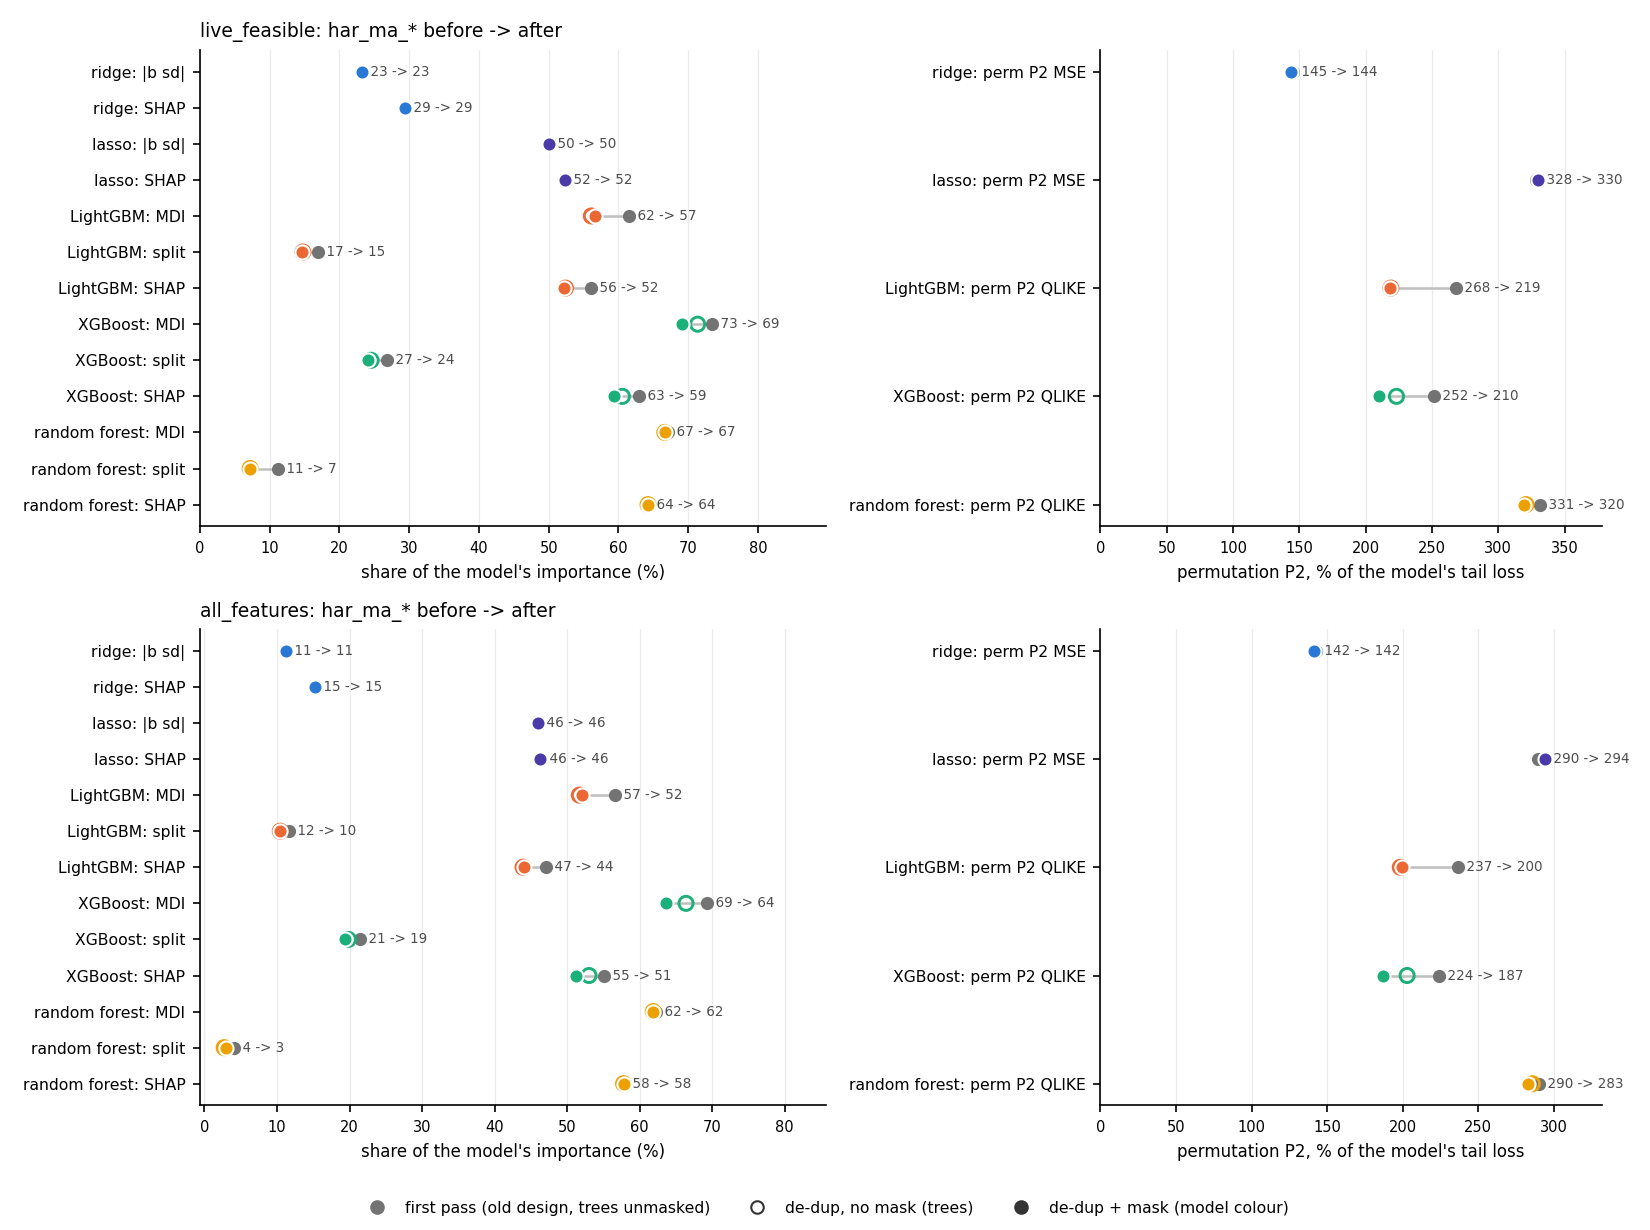
\includegraphics[width=\textwidth]{../results/feature_importance_1530_dedup/fig_before_after_har_ma.png}
\caption{\texttt{har\_ma\_*} before (old design) and after (de-dup + mask; open marker: de-dup, no mask), per model and measure; left: shares, right: permutation P2 as \% of the model's tail loss.}\end{figure}
\begin{figure}[H]\centering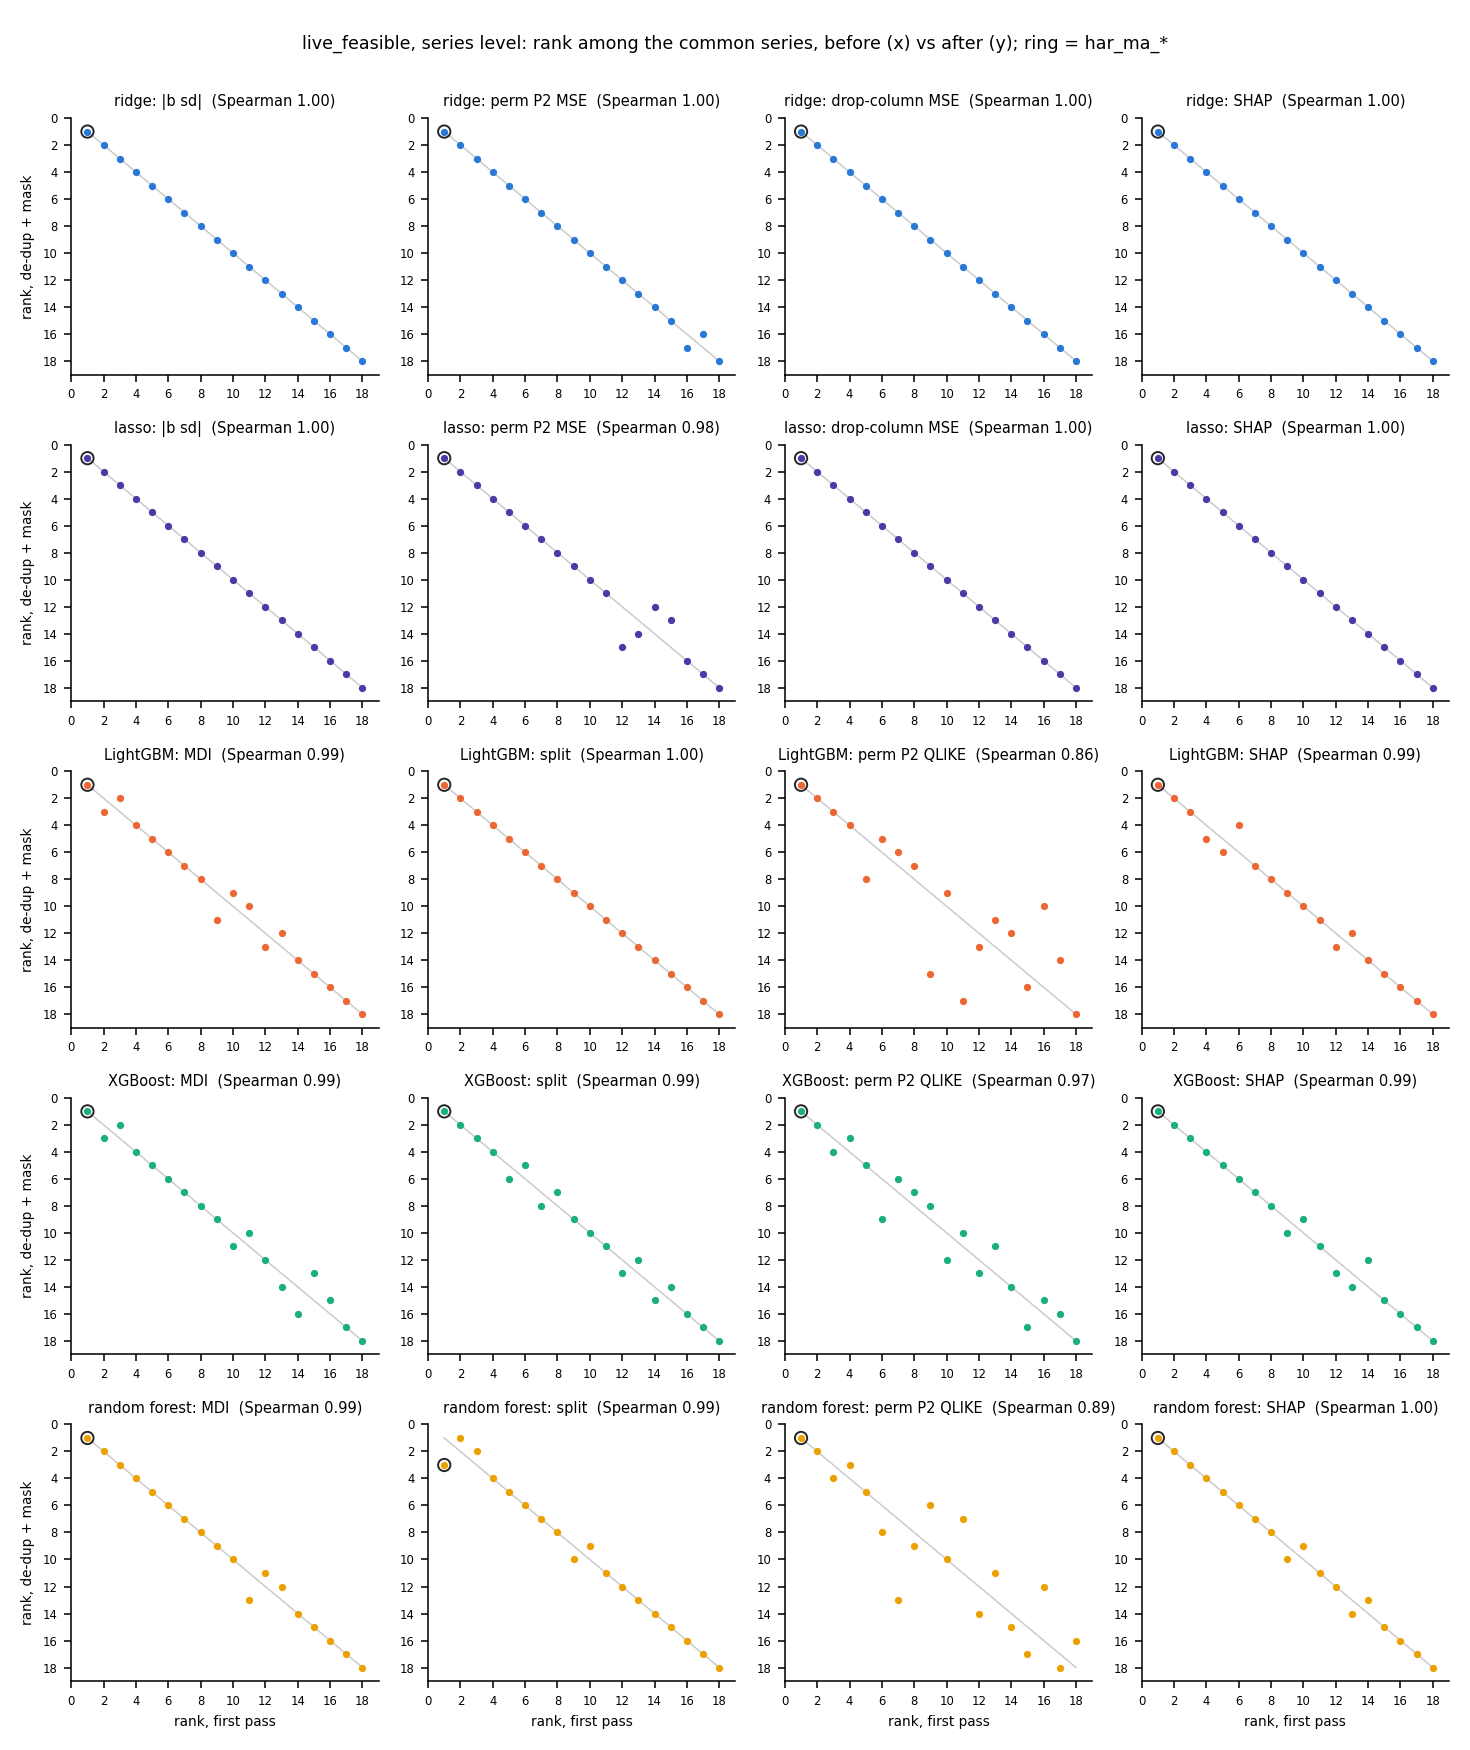
\includegraphics[width=\textwidth]{../results/feature_importance_1530_dedup/fig_before_after_ranks_live_feasible.png}
\caption{Live-feasible, series level: rank among the common series, old (x) vs new (y), per model and measure; on the diagonal = unchanged.}\end{figure}
\begin{itemize}\itemsep1pt
\item \texttt{har\_ma\_*} in the trees, live\_feasible: LightGBM MDI 62 $\to$ 57 \%, SHAP 56 $\to$ 52 \%, perm P2 dQLIKE +268 $\to$ +219 \% of tail loss (the old \texttt{\_x\_close} copies carried 29 \% of the old har\_ma column MDI); XGBoost MDI 73 $\to$ 69 \%, SHAP 63 $\to$ 59 \%, perm P2 dQLIKE +252 $\to$ +210 \% of tail loss (the old \texttt{\_x\_close} copies carried 22 \% of the old har\_ma column MDI); random forest MDI 67 $\to$ 67 \%, SHAP 64 $\to$ 64 \%, perm P2 dQLIKE +331 $\to$ +320 \% of tail loss (the old \texttt{\_x\_close} copies carried 49 \% of the old har\_ma column MDI).
\item \texttt{har\_ma\_*} in the trees, all\_features: LightGBM MDI 57 $\to$ 52 \%, SHAP 47 $\to$ 44 \%, perm P2 dQLIKE +237 $\to$ +200 \% of tail loss (the old \texttt{\_x\_close} copies carried 22 \% of the old har\_ma column MDI); XGBoost MDI 69 $\to$ 64 \%, SHAP 55 $\to$ 51 \%, perm P2 dQLIKE +224 $\to$ +187 \% of tail loss (the old \texttt{\_x\_close} copies carried 22 \% of the old har\_ma column MDI); random forest MDI 62 $\to$ 62 \%, SHAP 58 $\to$ 58 \%, perm P2 dQLIKE +290 $\to$ +283 \% of tail loss (the old \texttt{\_x\_close} copies carried 54 \% of the old har\_ma column MDI).
\item The draw-noise yardstick: the ridge fits are the same problem in both runs, so its \texttt{har\_ma\_*} change is the Monte Carlo of fresh permutation draws alone: perm P2 dMSE moves by at most 1.7 points of \% tail loss over the three buckets (abs(beta x sd), SHAP and drop-column unchanged).
\item Spearman old vs new (series level, common units, every bucket x measure): trees median 0.90 (min 0.66), linear median 1.00 (min 0.87); trees old vs de-dup no mask 0.94 (min 0.57), no mask vs mask 0.95 (min 0.66).
\item Spearman old vs new (cluster level, common units, every bucket x measure): trees median 0.93 (min 0.59), linear median 1.00 (min 0.77); trees old vs de-dup no mask 0.97 (min 0.56), no mask vs mask 0.97 (min 0.62).
\item Spearman old vs new (column level, common units, every bucket x measure): trees median 0.94 (min 0.38), linear median 1.00 (min 0.79); trees old vs de-dup no mask 0.97 (min 0.42), no mask vs mask 0.94 (min 0.40).
\item Series leader changed in 7 of 111 bucket x model x measure rows: live\_feasible ridge perm P1 QL \texttt{sumret4} $\to$ \texttt{sumabsret}; live\_feasible lasso perm P2 QL \texttt{har\_ma} $\to$ \texttt{vix3m}; live\_feasible random forest split \texttt{har\_ma} $\to$ \texttt{numobs}; all\_features ridge perm P1 QL \texttt{sumret4\_ewstock} $\to$ \texttt{sumautocov}; all\_features ridge perm P2 QL \texttt{sumautocov} $\to$ \texttt{voldemand\_spx\_open\_only}; all\_features lasso perm P2 QL \texttt{har\_ma} $\to$ \texttt{effspread\_vwstock}; all\_features random forest split \texttt{har\_ma} $\to$ \texttt{voldemand\_spx\_open\_and\_close}.
\item Clusters baseline: matched 19, removed (session-edge only) 6.
\item Clusters live\_feasible: matched 135, removed (session-edge only) 6.
\item Clusters all\_features: matched 230, removed (session-edge only) 6.
\item Column level, the dilution the copies caused (permutation P2 dQLIKE x 1e-3 of \texttt{har\_ma\_1} / \texttt{har\_ma\_5} alone, old $\to$ new; old = its \texttt{\_x\_close} copy left intact): live-feasible LightGBM 34.1 $\to$ 48.7 / 27.9 $\to$ 44.1; live-feasible XGBoost 34.3 $\to$ 49.7 / 34.2 $\to$ 43.8; live-feasible random forest 25.9 $\to$ 78.3 / 18.0 $\to$ 62.9; all features LightGBM 33.4 $\to$ 47.4 / 30.7 $\to$ 41.0; all features XGBoost 36.0 $\to$ 46.8 / 25.9 $\to$ 38.3; all features random forest 18.6 $\to$ 78.7 / 18.4 $\to$ 61.9.
\item ridge: perm P2 MSE: \texttt{fomc\_until\_inv} 16$\to$17, \texttt{fomc\_release} 17$\to$16
\item lasso: perm P2 MSE: \texttt{sumret3} 12$\to$15, \texttt{numobs} 14$\to$12
\item LightGBM: MDI: \texttt{calendar} 9$\to$11, \texttt{sumret} 2$\to$3; SHAP: \texttt{sumabsret} 6$\to$4, \texttt{calendar} 4$\to$5; perm P2 QL: \texttt{fomc\_since\_inv} 9$\to$15, \texttt{vix3m} 11$\to$17; perm P2 MSE: \texttt{sumabsret} 16$\to$5, \texttt{vix} 14$\to$10
\item XGBoost: MDI: \texttt{fomc\_since\_inv} 14$\to$16, \texttt{sumpret2} 15$\to$13; split: \texttt{numobs} 5$\to$6, \texttt{sumret3} 6$\to$5; SHAP: \texttt{fomc\_until\_inv} 14$\to$12, \texttt{vix} 9$\to$10; perm P2 QL: \texttt{sumautocov} 6$\to$9, \texttt{numobs} 10$\to$12; perm P2 MSE: \texttt{numobs} 8$\to$16, \texttt{fomc\_day} 12$\to$17
\item random forest: MDI: \texttt{calendar} 11$\to$13, \texttt{sumret4} 12$\to$11; split: \texttt{har\_ma} 1$\to$3, \texttt{numobs} 2$\to$1; SHAP: \texttt{numobs} 9$\to$10, \texttt{sumret4} 10$\to$9; perm P2 QL: \texttt{vix3m} 7$\to$13, \texttt{sumbipow} 11$\to$7; perm P2 MSE: \texttt{sumpret2} 6$\to$13, \texttt{vix3m} 7$\to$14
\item ridge: perm P2 MSE: \texttt{sumbipow\_vwstock} 21$\to$18, \texttt{sumvolume} 17$\to$19
\item lasso: perm P2 MSE: \texttt{sumbipow\_vwstock} 24$\to$20, \texttt{sumautocov} 20$\to$23
\item LightGBM: MDI: \texttt{sumret} 2$\to$3, \texttt{sumabsret} 3$\to$2; split: \texttt{sumabsret} 18$\to$9, \texttt{stocktwits\_sentcount} 13$\to$17; SHAP: \texttt{voldemand\_spx\_open\_and\_close} 28$\to$20, \texttt{sumret3\_ewstock} 18$\to$22; perm P2 QL: \texttt{sumautocov} 9$\to$40, \texttt{buyturnover\_ewstock} 12$\to$43; perm P2 MSE: \texttt{sumabsret} 33$\to$4, \texttt{fomc\_until\_inv} 36$\to$20
\item XGBoost: MDI: \texttt{sumbipow} 20$\to$15, \texttt{sumret3\_ewstock} 16$\to$19; split: \texttt{sumabsret} 8$\to$5, \texttt{sumret3} 7$\to$9; SHAP: \texttt{sumbipow} 17$\to$14, \texttt{turnover\_vwstock} 14$\to$16; perm P2 QL: \texttt{stocktwits\_sentcount} 28$\to$14, \texttt{sellturnover\_ewstock} 31$\to$18; perm P2 MSE: \texttt{vix3m} 30$\to$14, \texttt{voldemand\_all\_open\_only} 18$\to$31
\item random forest: MDI: \texttt{stocktwits\_sentcount} 17$\to$20, \texttt{sumret3\_ewstock} 19$\to$16; split: \texttt{sumret2\_ewstock} 36$\to$12, \texttt{vvix} 39$\to$20; SHAP: \texttt{buyturnover\_ewstock} 15$\to$18, \texttt{sumret3\_ewstock} 18$\to$15; perm P2 QL: \texttt{sumret3\_ewstock} 10$\to$29, \texttt{ofi\_ewstock} 28$\to$9; perm P2 MSE: \texttt{ofi\_vwstock} 13$\to$39, \texttt{vvix} 10$\to$33
\end{itemize}

\appendix
\section*{Appendix: HAR + calendar design}
\begin{table}[H]\centering\scriptsize
\caption{HAR + calendar, series level: top three per model and measure.}
\begin{tabular}{llp{11.2cm}}\toprule
model & measure & top three\\\midrule
ridge & $|\beta\cdot sd|$ & \texttt{har\_ma\_*} 81\%; \texttt{calendar} 19\% \\
ridge & perm.\ P1, $\Delta$MSE & \texttt{har\_ma\_*} +287\%; \texttt{calendar} +8\% \\
ridge & perm.\ P2, $\Delta$MSE & \texttt{har\_ma\_*} +501\%; \texttt{calendar} +9\% \\
ridge & perm.\ P2, $\Delta$QLIKE & \texttt{har\_ma\_*} +544\%; \texttt{calendar} +9\% \\
ridge & drop-column, $\Delta$MSE & \texttt{har\_ma\_*} +247\%; \texttt{calendar} +5\% \\
ridge & SHAP mean $|\phi|$ & \texttt{har\_ma\_*} 90\%; \texttt{calendar} 10\% \\
lasso & $|\beta\cdot sd|$ & \texttt{har\_ma\_*} 84\%; \texttt{calendar} 16\% \\
lasso & perm.\ P1, $\Delta$MSE & \texttt{har\_ma\_*} +284\%; \texttt{calendar} +7\% \\
lasso & perm.\ P2, $\Delta$MSE & \texttt{har\_ma\_*} +495\%; \texttt{calendar} +7\% \\
lasso & perm.\ P2, $\Delta$QLIKE & \texttt{har\_ma\_*} +544\%; \texttt{calendar} +9\% \\
lasso & drop-column, $\Delta$MSE & \texttt{har\_ma\_*} +244\%; \texttt{calendar} +4\% \\
lasso & SHAP mean $|\phi|$ & \texttt{har\_ma\_*} 91\%; \texttt{calendar} 9\% \\
LightGBM & MDI / gain & \texttt{har\_ma\_*} 95\%; \texttt{calendar} 5\% \\
LightGBM & split count & \texttt{har\_ma\_*} 85\%; \texttt{calendar} 15\% \\
LightGBM & perm.\ P1, $\Delta$QLIKE & \texttt{har\_ma\_*} +224\%; \texttt{calendar} +8\% \\
LightGBM & perm.\ P2, $\Delta$QLIKE & \texttt{har\_ma\_*} +488\%; \texttt{calendar} +8\% \\
LightGBM & perm.\ P2, $\Delta$MSE & \texttt{har\_ma\_*} +430\%; \texttt{calendar} +7\% \\
LightGBM & SHAP mean $|\phi|$ & \texttt{har\_ma\_*} 90\%; \texttt{calendar} 10\% \\
XGBoost & MDI / gain & \texttt{har\_ma\_*} 97\%; \texttt{calendar} 3\% \\
XGBoost & split count & \texttt{har\_ma\_*} 79\%; \texttt{calendar} 21\% \\
XGBoost & perm.\ P1, $\Delta$QLIKE & \texttt{har\_ma\_*} +218\%; \texttt{calendar} +6\% \\
XGBoost & perm.\ P2, $\Delta$QLIKE & \texttt{har\_ma\_*} +457\%; \texttt{calendar} +6\% \\
XGBoost & perm.\ P2, $\Delta$MSE & \texttt{har\_ma\_*} +444\%; \texttt{calendar} +4\% \\
XGBoost & SHAP mean $|\phi|$ & \texttt{har\_ma\_*} 93\%; \texttt{calendar} 7\% \\
random forest & MDI / gain & \texttt{har\_ma\_*} 95\%; \texttt{calendar} 5\% \\
random forest & split count & \texttt{har\_ma\_*} 76\%; \texttt{calendar} 24\% \\
random forest & perm.\ P1, $\Delta$QLIKE & \texttt{har\_ma\_*} +235\%; \texttt{calendar} +6\% \\
random forest & perm.\ P2, $\Delta$QLIKE & \texttt{har\_ma\_*} +527\%; \texttt{calendar} +6\% \\
random forest & perm.\ P2, $\Delta$MSE & \texttt{har\_ma\_*} +453\%; \texttt{calendar} +5\% \\
random forest & SHAP mean $|\phi|$ & \texttt{har\_ma\_*} 92\%; \texttt{calendar} 8\% \\
\bottomrule\end{tabular}\end{table}
\begin{figure}[H]\centering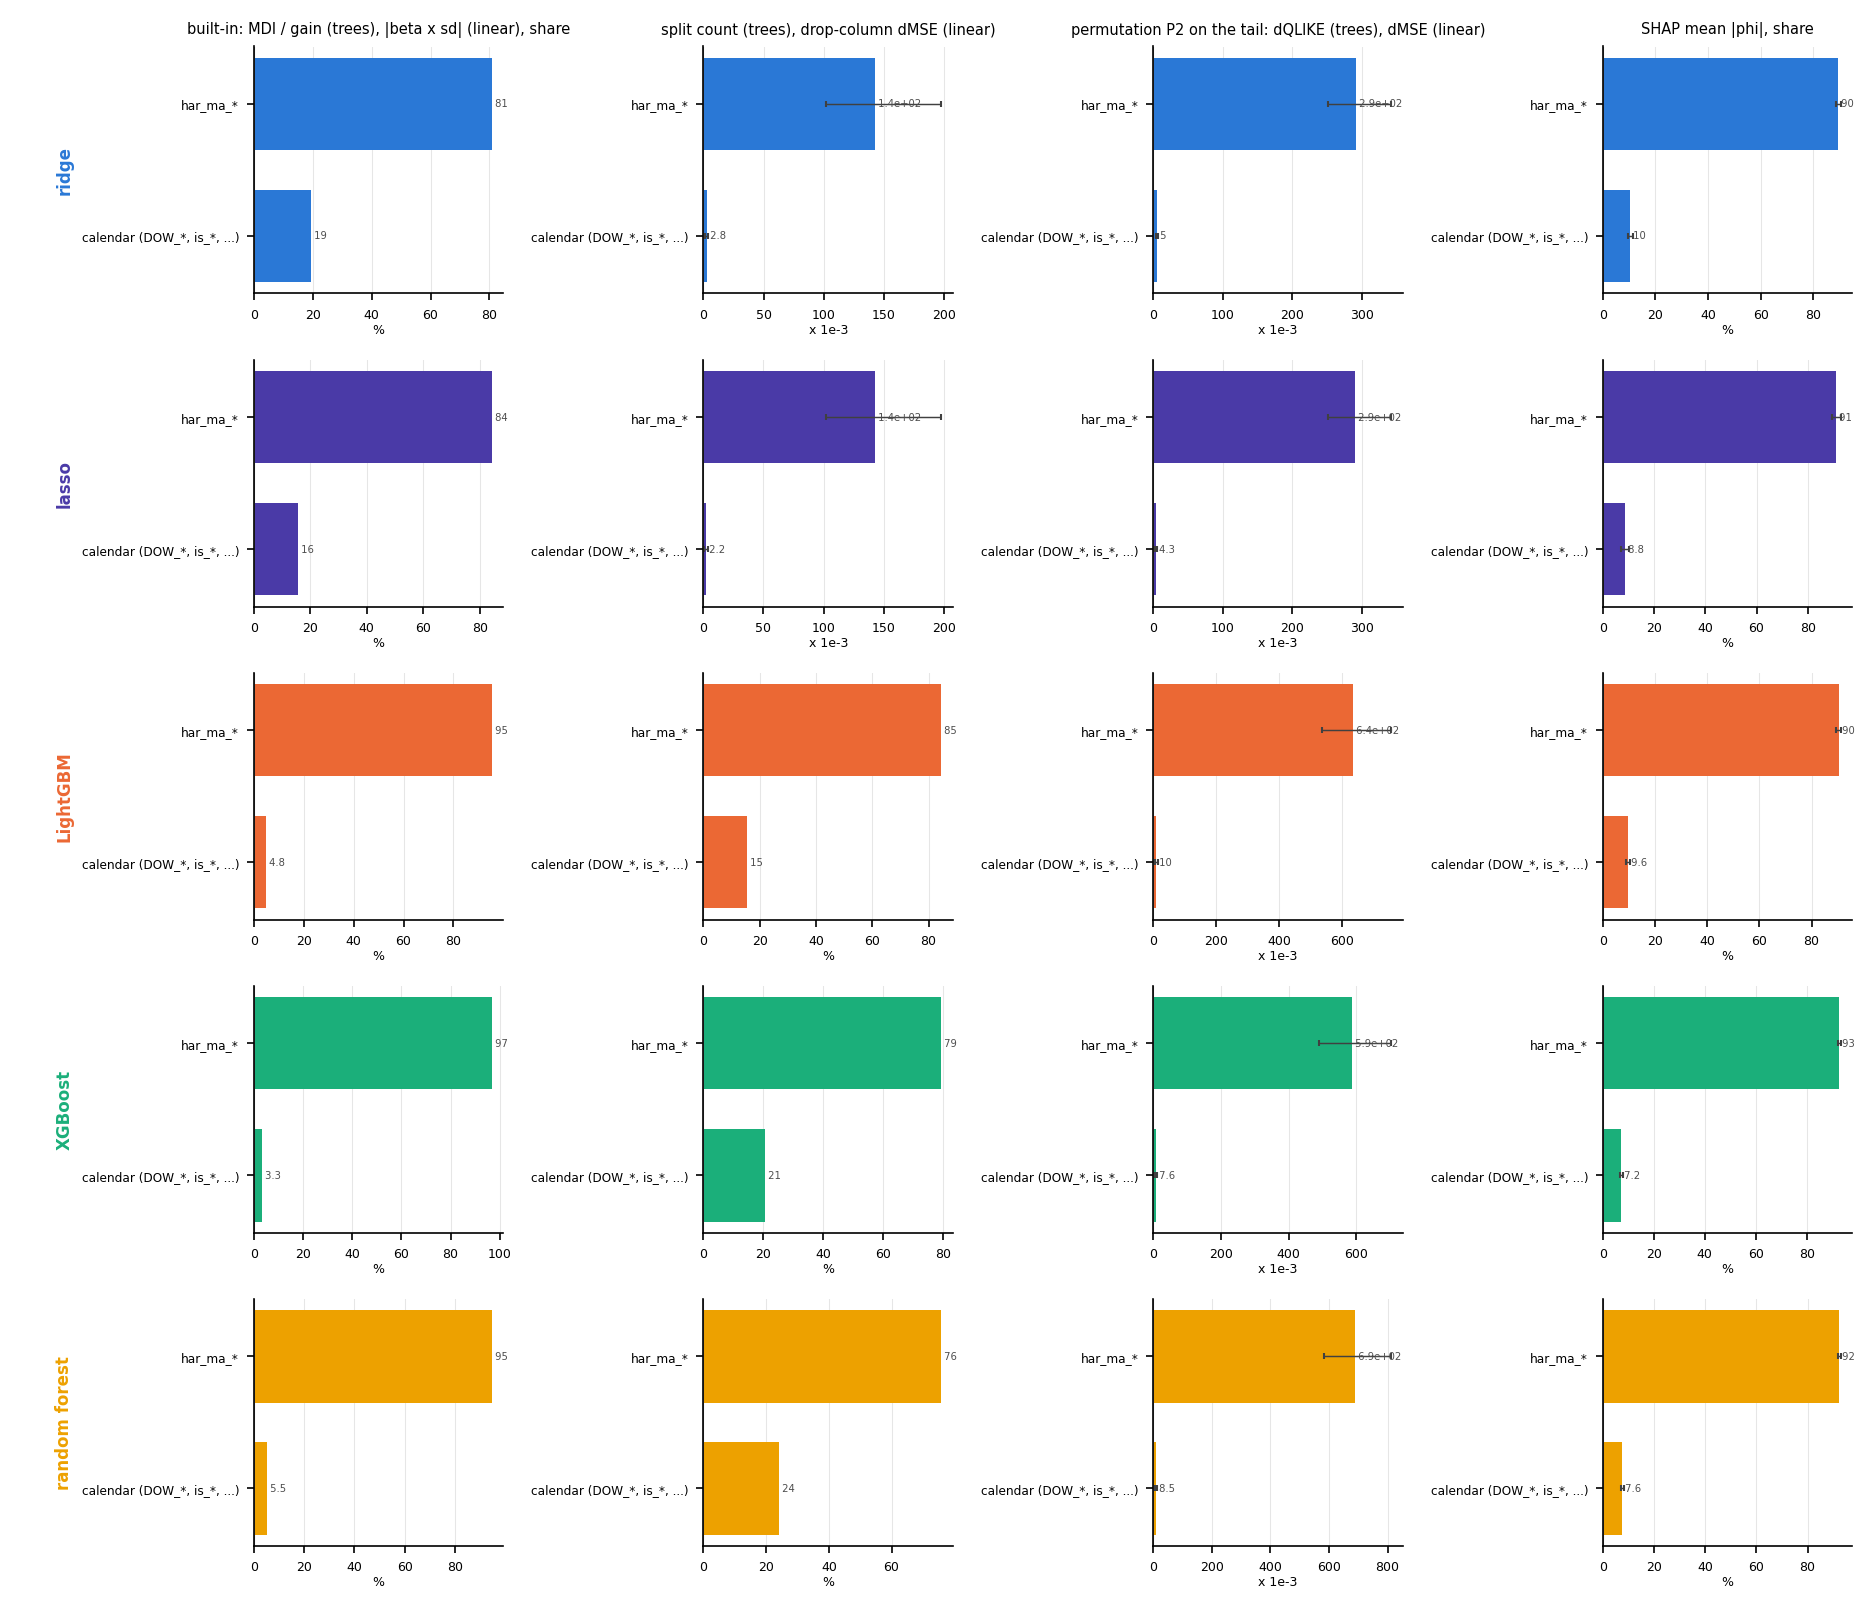
\includegraphics[width=\textwidth]{../results/feature_importance_1530_dedup/fig_ranked_baseline.png}
\caption{HAR + calendar: ranked bars per measure.}\end{figure}
\begin{figure}[H]\centering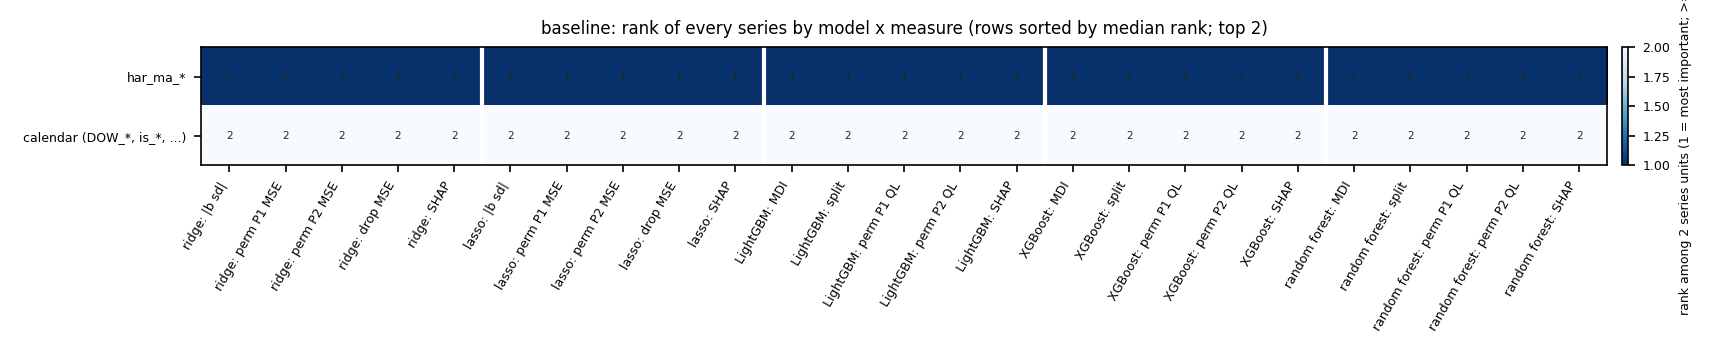
\includegraphics[width=0.7\textwidth]{../results/feature_importance_1530_dedup/fig_rank_heatmap_baseline_series.png}
\caption{HAR + calendar: ranks across measures.}\end{figure}
\begin{figure}[H]\centering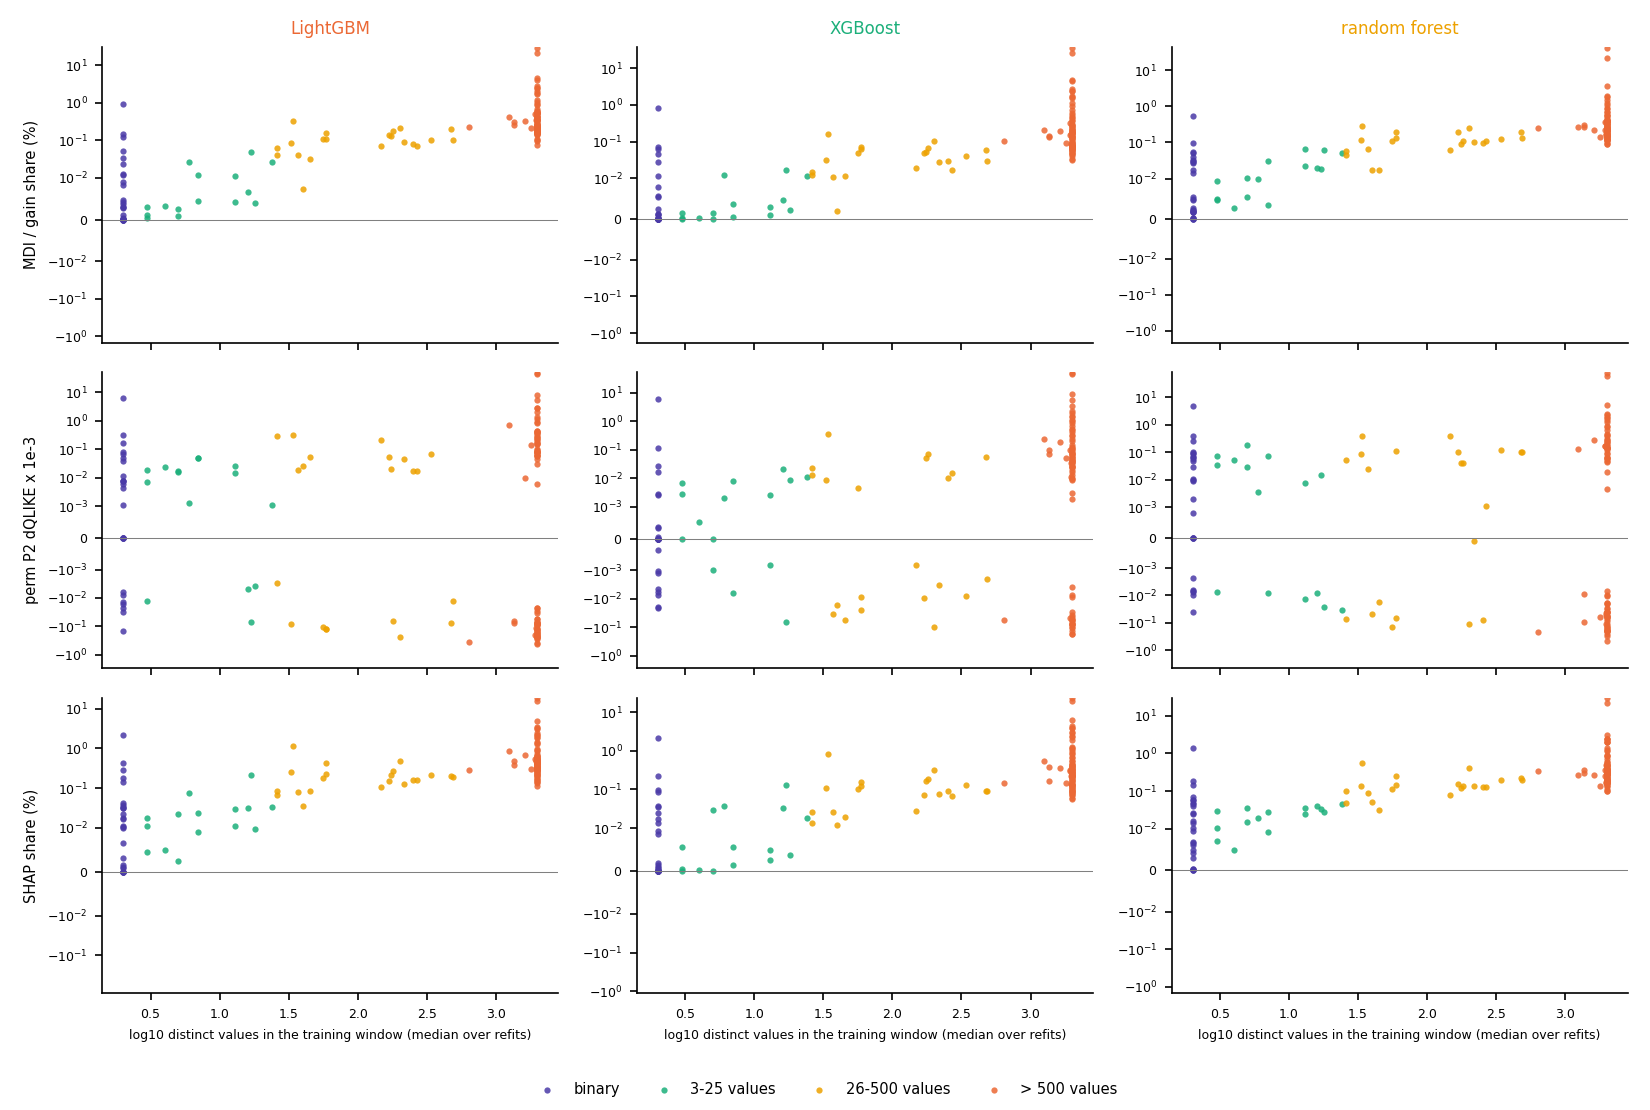
\includegraphics[width=\textwidth]{../results/feature_importance_1530_dedup/fig_cardinality_live_feasible.png}
\caption{Live-feasible columns: MDI share, permutation P2 $\Delta$QLIKE and SHAP share against the number of distinct values in the training window (log scale), by cardinality class.}\end{figure}
\begin{figure}[H]\centering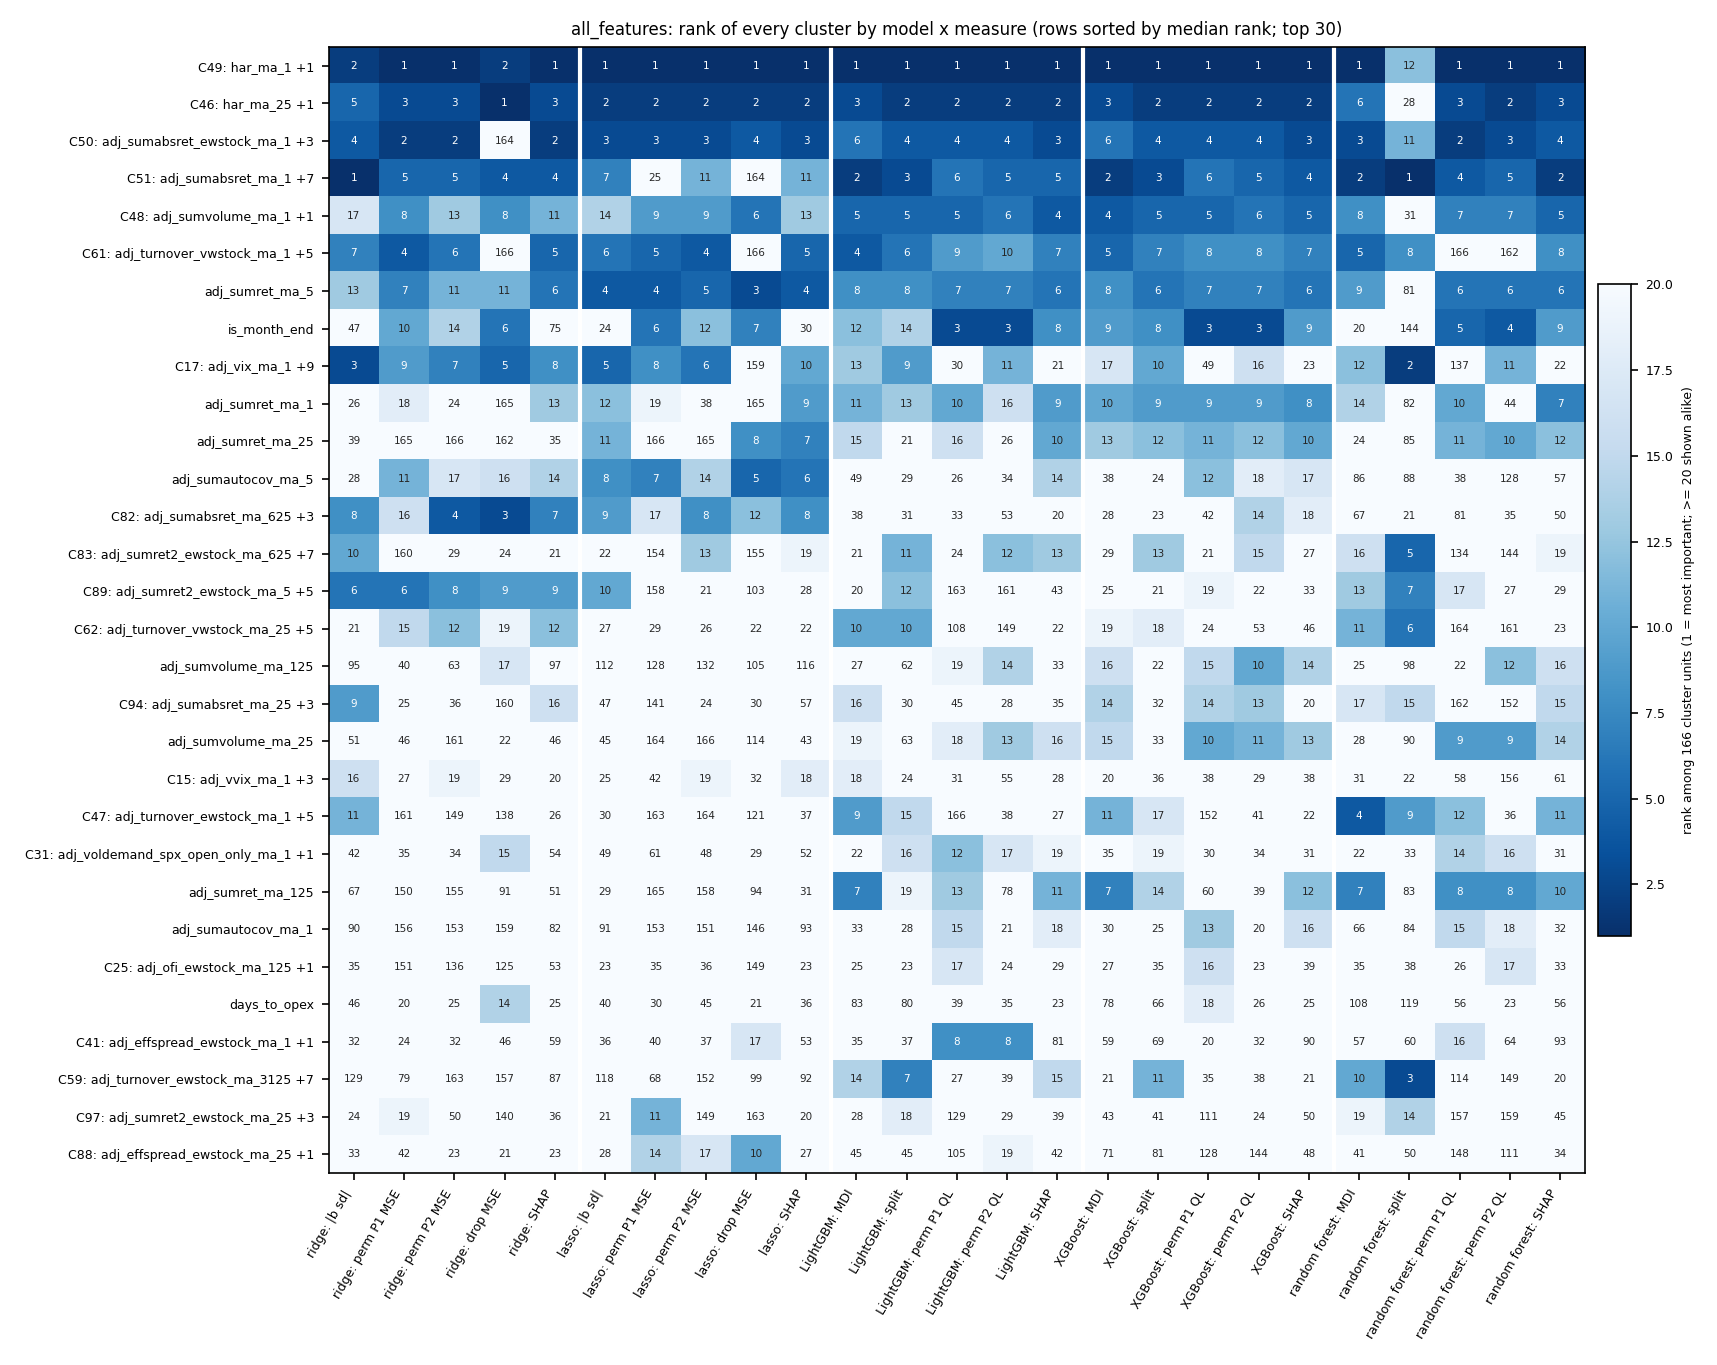
\includegraphics[width=0.95\textwidth]{../results/feature_importance_1530_dedup/fig_rank_heatmap_all_features_cluster.png}
\caption{All features: ranks at the cluster level.}\end{figure}

\end{document}
